% Options for packages loaded elsewhere
\PassOptionsToPackage{unicode}{hyperref}
\PassOptionsToPackage{hyphens}{url}
%
\documentclass[
]{book}
\usepackage{amsmath,amssymb}
\usepackage{lmodern}
\usepackage{iftex}
\ifPDFTeX
  \usepackage[T1]{fontenc}
  \usepackage[utf8]{inputenc}
  \usepackage{textcomp} % provide euro and other symbols
\else % if luatex or xetex
  \usepackage{unicode-math}
  \defaultfontfeatures{Scale=MatchLowercase}
  \defaultfontfeatures[\rmfamily]{Ligatures=TeX,Scale=1}
\fi
% Use upquote if available, for straight quotes in verbatim environments
\IfFileExists{upquote.sty}{\usepackage{upquote}}{}
\IfFileExists{microtype.sty}{% use microtype if available
  \usepackage[]{microtype}
  \UseMicrotypeSet[protrusion]{basicmath} % disable protrusion for tt fonts
}{}
\makeatletter
\@ifundefined{KOMAClassName}{% if non-KOMA class
  \IfFileExists{parskip.sty}{%
    \usepackage{parskip}
  }{% else
    \setlength{\parindent}{0pt}
    \setlength{\parskip}{6pt plus 2pt minus 1pt}}
}{% if KOMA class
  \KOMAoptions{parskip=half}}
\makeatother
\usepackage{xcolor}
\usepackage{color}
\usepackage{fancyvrb}
\newcommand{\VerbBar}{|}
\newcommand{\VERB}{\Verb[commandchars=\\\{\}]}
\DefineVerbatimEnvironment{Highlighting}{Verbatim}{commandchars=\\\{\}}
% Add ',fontsize=\small' for more characters per line
\usepackage{framed}
\definecolor{shadecolor}{RGB}{248,248,248}
\newenvironment{Shaded}{\begin{snugshade}}{\end{snugshade}}
\newcommand{\AlertTok}[1]{\textcolor[rgb]{0.94,0.16,0.16}{#1}}
\newcommand{\AnnotationTok}[1]{\textcolor[rgb]{0.56,0.35,0.01}{\textbf{\textit{#1}}}}
\newcommand{\AttributeTok}[1]{\textcolor[rgb]{0.77,0.63,0.00}{#1}}
\newcommand{\BaseNTok}[1]{\textcolor[rgb]{0.00,0.00,0.81}{#1}}
\newcommand{\BuiltInTok}[1]{#1}
\newcommand{\CharTok}[1]{\textcolor[rgb]{0.31,0.60,0.02}{#1}}
\newcommand{\CommentTok}[1]{\textcolor[rgb]{0.56,0.35,0.01}{\textit{#1}}}
\newcommand{\CommentVarTok}[1]{\textcolor[rgb]{0.56,0.35,0.01}{\textbf{\textit{#1}}}}
\newcommand{\ConstantTok}[1]{\textcolor[rgb]{0.00,0.00,0.00}{#1}}
\newcommand{\ControlFlowTok}[1]{\textcolor[rgb]{0.13,0.29,0.53}{\textbf{#1}}}
\newcommand{\DataTypeTok}[1]{\textcolor[rgb]{0.13,0.29,0.53}{#1}}
\newcommand{\DecValTok}[1]{\textcolor[rgb]{0.00,0.00,0.81}{#1}}
\newcommand{\DocumentationTok}[1]{\textcolor[rgb]{0.56,0.35,0.01}{\textbf{\textit{#1}}}}
\newcommand{\ErrorTok}[1]{\textcolor[rgb]{0.64,0.00,0.00}{\textbf{#1}}}
\newcommand{\ExtensionTok}[1]{#1}
\newcommand{\FloatTok}[1]{\textcolor[rgb]{0.00,0.00,0.81}{#1}}
\newcommand{\FunctionTok}[1]{\textcolor[rgb]{0.00,0.00,0.00}{#1}}
\newcommand{\ImportTok}[1]{#1}
\newcommand{\InformationTok}[1]{\textcolor[rgb]{0.56,0.35,0.01}{\textbf{\textit{#1}}}}
\newcommand{\KeywordTok}[1]{\textcolor[rgb]{0.13,0.29,0.53}{\textbf{#1}}}
\newcommand{\NormalTok}[1]{#1}
\newcommand{\OperatorTok}[1]{\textcolor[rgb]{0.81,0.36,0.00}{\textbf{#1}}}
\newcommand{\OtherTok}[1]{\textcolor[rgb]{0.56,0.35,0.01}{#1}}
\newcommand{\PreprocessorTok}[1]{\textcolor[rgb]{0.56,0.35,0.01}{\textit{#1}}}
\newcommand{\RegionMarkerTok}[1]{#1}
\newcommand{\SpecialCharTok}[1]{\textcolor[rgb]{0.00,0.00,0.00}{#1}}
\newcommand{\SpecialStringTok}[1]{\textcolor[rgb]{0.31,0.60,0.02}{#1}}
\newcommand{\StringTok}[1]{\textcolor[rgb]{0.31,0.60,0.02}{#1}}
\newcommand{\VariableTok}[1]{\textcolor[rgb]{0.00,0.00,0.00}{#1}}
\newcommand{\VerbatimStringTok}[1]{\textcolor[rgb]{0.31,0.60,0.02}{#1}}
\newcommand{\WarningTok}[1]{\textcolor[rgb]{0.56,0.35,0.01}{\textbf{\textit{#1}}}}
\usepackage{longtable,booktabs,array}
\usepackage{calc} % for calculating minipage widths
% Correct order of tables after \paragraph or \subparagraph
\usepackage{etoolbox}
\makeatletter
\patchcmd\longtable{\par}{\if@noskipsec\mbox{}\fi\par}{}{}
\makeatother
% Allow footnotes in longtable head/foot
\IfFileExists{footnotehyper.sty}{\usepackage{footnotehyper}}{\usepackage{footnote}}
\makesavenoteenv{longtable}
\usepackage{graphicx}
\makeatletter
\def\maxwidth{\ifdim\Gin@nat@width>\linewidth\linewidth\else\Gin@nat@width\fi}
\def\maxheight{\ifdim\Gin@nat@height>\textheight\textheight\else\Gin@nat@height\fi}
\makeatother
% Scale images if necessary, so that they will not overflow the page
% margins by default, and it is still possible to overwrite the defaults
% using explicit options in \includegraphics[width, height, ...]{}
\setkeys{Gin}{width=\maxwidth,height=\maxheight,keepaspectratio}
% Set default figure placement to htbp
\makeatletter
\def\fps@figure{htbp}
\makeatother
\setlength{\emergencystretch}{3em} % prevent overfull lines
\providecommand{\tightlist}{%
  \setlength{\itemsep}{0pt}\setlength{\parskip}{0pt}}
\setcounter{secnumdepth}{5}
\usepackage{booktabs}
\ifLuaTeX
  \usepackage{selnolig}  % disable illegal ligatures
\fi
\usepackage[]{natbib}
\bibliographystyle{apalike}
\IfFileExists{bookmark.sty}{\usepackage{bookmark}}{\usepackage{hyperref}}
\IfFileExists{xurl.sty}{\usepackage{xurl}}{} % add URL line breaks if available
\urlstyle{same} % disable monospaced font for URLs
\hypersetup{
  pdftitle={Einführung in R},
  pdfauthor={Stephan Goerigk},
  hidelinks,
  pdfcreator={LaTeX via pandoc}}

\title{Einführung in R}
\author{Stephan Goerigk}
\date{2022-11-19}

\begin{document}
\maketitle

{
\setcounter{tocdepth}{1}
\tableofcontents
}
\hypertarget{packages}{%
\chapter{Packages}\label{packages}}

You will need to install and load the following packages for these exercises:

\begin{Shaded}
\begin{Highlighting}[]
\CommentTok{\# install.packages("BayesFactor")}
\CommentTok{\# install.packages("MASS")}
\CommentTok{\# install.packages("devtools") \# if not yet installed}
\CommentTok{\# library(devtools)}
\CommentTok{\# install\_github("nicebread/BFDA", subdir="package")}
\CommentTok{\# }
\CommentTok{\# library(BFDA)}
\CommentTok{\# library(BayesFactor)}
\CommentTok{\# library(MASS)}

\CommentTok{\#Plus BFDA {-} see next section}
\end{Highlighting}
\end{Shaded}

\begin{Shaded}
\begin{Highlighting}[]
\CommentTok{\# install.packages("ggplot2")}
\CommentTok{\# install.packages("lme4")}
\CommentTok{\# install.packages("lmerTest")}
\CommentTok{\# install.packages("dendextend")}
\CommentTok{\# install.packages("tidyverse")}
\CommentTok{\# install.packages("lcmm")}
\CommentTok{\# install.packages("LCTMtools")}
\CommentTok{\# install.packages("cowplot")}
\CommentTok{\# install.packages("emmeans")}
\CommentTok{\# install.packages("psych")}
\CommentTok{\# install.packages("BBmisc")}

\FunctionTok{library}\NormalTok{(ggplot2)}
\FunctionTok{library}\NormalTok{(lme4)}
\FunctionTok{library}\NormalTok{(lmerTest)}
\FunctionTok{library}\NormalTok{(dendextend)}
\FunctionTok{library}\NormalTok{(tidyverse)}
\FunctionTok{library}\NormalTok{(lcmm)}
\FunctionTok{library}\NormalTok{(LCTMtools)}
\FunctionTok{library}\NormalTok{(cowplot)}
\FunctionTok{library}\NormalTok{(emmeans)}
\FunctionTok{library}\NormalTok{(psych)}
\FunctionTok{library}\NormalTok{(BBmisc)}
\end{Highlighting}
\end{Shaded}

\hypertarget{trial-design}{%
\chapter{Trial Design}\label{trial-design}}

\hypertarget{exercise-1-simulating-data-using-bfda-and-selecting-trial-parameters}{%
\section{Exercise 1: Simulating data using BFDA and selecting trial parameters}\label{exercise-1-simulating-data-using-bfda-and-selecting-trial-parameters}}

The Bayes factor design analysis (BFDA) package provides a simple way to simulate and analyse sequential bayesian analyses for trial planning. For more complex analyses you can create your own custom simulations (e.g.~see the scripts at \url{https://osf.io/8mxda/} for example)

Please see \url{https://rawgit.com/nicebread/BFDA/master/package/doc/BFDA_manual.html} for the BFDA manual and full instructions

\hypertarget{simulate-sequential-analyses-for-planning}{%
\subsection{Simulate sequential analyses for planning}\label{simulate-sequential-analyses-for-planning}}

A first step is to simulate the results of sequential analyses under i) the alternative hypothesis for the target effect size of interest (to find parameters that give you sufficient power), and ii) the null hypothesis (to find parameters that give a suitable false-positive (Type 1) error rate). Once you have suitable parameters for these, you can then simulate a range of other effect sizes to get a better picture of your power at different effect sizes.

As simulations can take some time, for demonstration purposes in this exercise we will i) attempt to find a medium effect size (d = 0.5), as this requires smaller maximum sample sizes, and ii) only do a small number of simulations (500), as we are not too worried about accuracy/precision - for planning an actual trial you would want to do a larger number (e.g.~10,000)

Please run the following simulations as preparation:

\begin{Shaded}
\begin{Highlighting}[]
\FunctionTok{set.seed}\NormalTok{(}\DecValTok{19112022}\NormalTok{)}

\NormalTok{sim.H1 }\OtherTok{\textless{}{-}} \FunctionTok{BFDA.sim}\NormalTok{(}\AttributeTok{expected.ES=}\FloatTok{0.5}\NormalTok{, }\AttributeTok{type=}\StringTok{"t.between"}\NormalTok{,}\AttributeTok{prior=}\FunctionTok{list}\NormalTok{(}\StringTok{"Cauchy"}\NormalTok{,}\FunctionTok{list}\NormalTok{(}\AttributeTok{prior.location=}\DecValTok{0}\NormalTok{, }\AttributeTok{prior.scale=}\FunctionTok{sqrt}\NormalTok{(}\DecValTok{2}\NormalTok{)}\SpecialCharTok{/}\DecValTok{2}\NormalTok{)), }\AttributeTok{n.min=}\DecValTok{10}\NormalTok{, }\AttributeTok{n.max=}\DecValTok{80}\NormalTok{, }\AttributeTok{alternative=}\StringTok{"greater"}\NormalTok{, }\AttributeTok{boundary=}\ConstantTok{Inf}\NormalTok{, }\AttributeTok{B=}\DecValTok{500}\NormalTok{, }\AttributeTok{verbose=}\ConstantTok{TRUE}\NormalTok{, }\AttributeTok{stepsize =} \DecValTok{5}\NormalTok{)}

\NormalTok{sim.H0 }\OtherTok{\textless{}{-}} \FunctionTok{BFDA.sim}\NormalTok{(}\AttributeTok{expected.ES=}\DecValTok{0}\NormalTok{, }\AttributeTok{type=}\StringTok{"t.between"}\NormalTok{, }\AttributeTok{prior=}\FunctionTok{list}\NormalTok{(}\StringTok{"Cauchy"}\NormalTok{, }\FunctionTok{list}\NormalTok{(}\AttributeTok{prior.location=}\DecValTok{0}\NormalTok{, }\AttributeTok{prior.scale=}\FunctionTok{sqrt}\NormalTok{(}\DecValTok{2}\NormalTok{)}\SpecialCharTok{/}\DecValTok{2}\NormalTok{)), }\AttributeTok{n.min=}\DecValTok{10}\NormalTok{, }\AttributeTok{n.max=}\DecValTok{80}\NormalTok{, }\AttributeTok{alternative=}\StringTok{"greater"}\NormalTok{, }\AttributeTok{boundary=}\ConstantTok{Inf}\NormalTok{, }\AttributeTok{B=}\DecValTok{500}\NormalTok{, }\AttributeTok{verbose=}\ConstantTok{TRUE}\NormalTok{, }\AttributeTok{stepsize =} \DecValTok{5}\NormalTok{)}

\CommentTok{\#if you notice these have finished and you have time you could also run some in{-}between or larger values, e.g.}

\NormalTok{sim.H0}\FloatTok{.2} \OtherTok{\textless{}{-}} \FunctionTok{BFDA.sim}\NormalTok{(}\AttributeTok{expected.ES=}\FloatTok{0.2}\NormalTok{, }\AttributeTok{type=}\StringTok{"t.between"}\NormalTok{, }\AttributeTok{prior=}\FunctionTok{list}\NormalTok{(}\StringTok{"Cauchy"}\NormalTok{, }\FunctionTok{list}\NormalTok{(}\AttributeTok{prior.location=}\DecValTok{0}\NormalTok{, }\AttributeTok{prior.scale=}\FunctionTok{sqrt}\NormalTok{(}\DecValTok{2}\NormalTok{)}\SpecialCharTok{/}\DecValTok{2}\NormalTok{)), }\AttributeTok{n.min=}\DecValTok{10}\NormalTok{, }\AttributeTok{n.max=}\DecValTok{80}\NormalTok{, }\AttributeTok{alternative=}\StringTok{"greater"}\NormalTok{, }\AttributeTok{boundary=}\ConstantTok{Inf}\NormalTok{, }\AttributeTok{B=}\DecValTok{500}\NormalTok{, }\AttributeTok{verbose=}\ConstantTok{TRUE}\NormalTok{, }\AttributeTok{stepsize =} \DecValTok{5}\NormalTok{)}

\NormalTok{sim.H0}\FloatTok{.4} \OtherTok{\textless{}{-}} \FunctionTok{BFDA.sim}\NormalTok{(}\AttributeTok{expected.ES=}\FloatTok{0.4}\NormalTok{, }\AttributeTok{type=}\StringTok{"t.between"}\NormalTok{, }\AttributeTok{prior=}\FunctionTok{list}\NormalTok{(}\StringTok{"Cauchy"}\NormalTok{, }\FunctionTok{list}\NormalTok{(}\AttributeTok{prior.location=}\DecValTok{0}\NormalTok{, }\AttributeTok{prior.scale=}\FunctionTok{sqrt}\NormalTok{(}\DecValTok{2}\NormalTok{)}\SpecialCharTok{/}\DecValTok{2}\NormalTok{)), }\AttributeTok{n.min=}\DecValTok{10}\NormalTok{, }\AttributeTok{n.max=}\DecValTok{80}\NormalTok{, }\AttributeTok{alternative=}\StringTok{"greater"}\NormalTok{, }\AttributeTok{boundary=}\ConstantTok{Inf}\NormalTok{, }\AttributeTok{B=}\DecValTok{500}\NormalTok{, }\AttributeTok{verbose=}\ConstantTok{TRUE}\NormalTok{, }\AttributeTok{stepsize =} \DecValTok{5}\NormalTok{)}

\NormalTok{sim.H0}\FloatTok{.6} \OtherTok{\textless{}{-}} \FunctionTok{BFDA.sim}\NormalTok{(}\AttributeTok{expected.ES=}\FloatTok{0.6}\NormalTok{, }\AttributeTok{type=}\StringTok{"t.between"}\NormalTok{, }\AttributeTok{prior=}\FunctionTok{list}\NormalTok{(}\StringTok{"Cauchy"}\NormalTok{, }\FunctionTok{list}\NormalTok{(}\AttributeTok{prior.location=}\DecValTok{0}\NormalTok{, }\AttributeTok{prior.scale=}\FunctionTok{sqrt}\NormalTok{(}\DecValTok{2}\NormalTok{)}\SpecialCharTok{/}\DecValTok{2}\NormalTok{)), }\AttributeTok{n.min=}\DecValTok{10}\NormalTok{, }\AttributeTok{n.max=}\DecValTok{80}\NormalTok{, }\AttributeTok{alternative=}\StringTok{"greater"}\NormalTok{, }\AttributeTok{boundary=}\ConstantTok{Inf}\NormalTok{, }\AttributeTok{B=}\DecValTok{500}\NormalTok{, }\AttributeTok{verbose=}\ConstantTok{TRUE}\NormalTok{, }\AttributeTok{stepsize =} \DecValTok{5}\NormalTok{)}

\CommentTok{\#etc...}
\end{Highlighting}
\end{Shaded}

As an explanation, these simulate sequential Bayes-factor based analyses based on:

\begin{enumerate}
\def\labelenumi{\alph{enumi})}
\item
  Effect size of d = 0.5 (expected.ES=0.5) for sim.H1, or d=0 for sim.H0
\item
  a between-group t-test, e.g.~difference between two groups in change in symptoms (type=``t.between'')
\item
  use a default Cauchy prior with a rscale value of 0.707 (prior=list(``Cauchy'', list(prior.location=0, prior.scale=sqrt(2)/2))) {[}we can't go into priors today but default ones like this work fine! See Stefan et al.~(2019) for discussion of using informed priors with BFDA, \url{https://link.springer.com/article/10.3758/s13428-018-01189-8}{]}
\item
  a minimum sample size (per arm) of 10 (n.min = 10) - note that when trying to find parameters later you can choose higher minimum sample sizes, but not lower
\item
  a maximum sample size (per arm) of 80 (n.max = 80) - note that when trying out parameters later on you can try lower, but not higher maximum sample sizes
\item
  a directional (i.e.~one-tailed) Bayes Factor (alternative = ``greater'' and boundary = Inf). We are interested in whether one treatment is superior to another, not whether it is different.
\item
  we use 500 simulations (B = 500) - fine for getting a feel, but for finalising your study design you would want a larger number e.g.~10,000
\item
  we carry out the analysis every 5 participants (stepsize = 5). You can repeat the analysis every 1 participant, but this simply takes longer to simulate so we don't do this here.
\end{enumerate}

If you were carrying out large important simulations that took a long time you would probably want to save them so that you can load them again later without having to re-run the simulations:

\begin{Shaded}
\begin{Highlighting}[]
\CommentTok{\#Saving a BFDA simulation object:}
\FunctionTok{saveRDS}\NormalTok{(sim.H1,}\StringTok{"sim.H1.d0.5.dd.mm.yy.RDS"}\NormalTok{)}
\FunctionTok{saveRDS}\NormalTok{(sim.H0,}\StringTok{"sim.H1.d0.0.dd.mm.yy.RDS"}\NormalTok{)}
\CommentTok{\#to load again}
\NormalTok{sim.H1}\OtherTok{\textless{}{-}}\FunctionTok{readRDS}\NormalTok{(}\StringTok{"sim.H1.d0.5.dd.mm.yy.RDS"}\NormalTok{)}
\NormalTok{sim.H0}\OtherTok{\textless{}{-}}\FunctionTok{readRDS}\NormalTok{(}\StringTok{"sim.H1.d0.0.dd.mm.yy.RDS"}\NormalTok{)}
\end{Highlighting}
\end{Shaded}

\hypertarget{try-out-different-analysis-parameters-to-find-a-set-that-fits-your-requirements}{%
\subsection{Try out different analysis parameters to find a set that fits your requirements}\label{try-out-different-analysis-parameters-to-find-a-set-that-fits-your-requirements}}

\hypertarget{overview}{%
\subsubsection{Overview}\label{overview}}

Now that you have a simulated set of sequential BFs you can test out what would happen if you applied different sets of analysis parameters to them.

These are:

\begin{itemize}
\item
  Nmin: The minimum sample size (per arm) at which you start the sequential analyses
\item
  Nmax: The maximum sample size (per arm) at which you drop an arm (if it has not already hit a BF boundary)
\item
  BFfail: A BF threshold for failure (i.e.~sufficient evidence for the null hypothesis of non-superiority to the control condition vs.~the alternative hypothesis of superiority). This will be a value less than 1 (e.g.~1/3, 1/5, 1/10 etc)
\item
  BFsuccess: A BF threshold for success (i.e.~sufficient evidence for the alternative hypothesis of superiority over the control condition vs.the null hypothesis of non-superiority to the control condition ). This will be a value greater than 1 (e.g.~3, 5, 10)
\end{itemize}

We are interested in:

\begin{enumerate}
\def\labelenumi{\roman{enumi})}
\item
  power: what proportion of arms hit the BFsuccess threshold when d \textgreater{} 0
\item
  false-positive / Type 1 error rate: what proportion of arms hit BF success threshold when d = 0 (or d \textless{} 0)
\item
  keeping the average sample sizes as low as possible
\end{enumerate}

There are several functions in BFDA to analyse simulation outcomes, but here we will just use the plot function. We will start by using the boundary conditions of the simulations (i.e.~n.min = 10 and n.max = 80), and a default set of starting boundaries of BFfail = 1/5 and BFsuccess = 5 (boundary=c(1/5, 5)). The parameter n.trajectories just tells it how many lines to draw on the graph (representing individual BF trajectories)

\begin{Shaded}
\begin{Highlighting}[]
\CommentTok{\#First plot for H1}
\FunctionTok{dev.new}\NormalTok{() }\CommentTok{\#sometimes the plot doesn\textquotesingle{}t work if you don\textquotesingle{}t make a new window first}
\FunctionTok{plot}\NormalTok{(sim.H1, }\AttributeTok{n.min=}\DecValTok{10}\NormalTok{, }\AttributeTok{n.max=}\DecValTok{80}\NormalTok{, }\AttributeTok{boundary=}\FunctionTok{c}\NormalTok{(}\DecValTok{1}\SpecialCharTok{/}\DecValTok{5}\NormalTok{, }\DecValTok{5}\NormalTok{), }\AttributeTok{n.trajectories =} \DecValTok{60}\NormalTok{)}

\CommentTok{\#Then plot for H0}
\FunctionTok{dev.new}\NormalTok{() }\CommentTok{\#sometimes the plot doesn\textquotesingle{}t work if you don\textquotesingle{}t make a new window first}
\FunctionTok{plot}\NormalTok{(sim.H0, }\AttributeTok{n.min=}\DecValTok{10}\NormalTok{, }\AttributeTok{n.max=}\DecValTok{80}\NormalTok{, }\AttributeTok{boundary=}\FunctionTok{c}\NormalTok{(}\DecValTok{1}\SpecialCharTok{/}\DecValTok{5}\NormalTok{, }\DecValTok{5}\NormalTok{), }\AttributeTok{n.trajectories =} \DecValTok{60}\NormalTok{)}

\CommentTok{\#There are other functions in BFDA to explore the simulations/sequential analyses but I find the plots the most informative. However, feel free to explore.}
\end{Highlighting}
\end{Shaded}

\hypertarget{exercise-steps}{%
\subsubsection{Exercise steps}\label{exercise-steps}}

\begin{enumerate}
\def\labelenumi{\arabic{enumi}.}
\item
  Play around with the parameters (n.min, n.max, the BF boundaries) and see what happens. e.g.~increasing n.min will tend to reduce error rates, but means you lose the chance to make decisions so quickly. Remember that the BF boundaries don't have to be symmetrical (e.g.~you could use boundary=c(1/3,10) if you weren't so worried about false-negatives but were very concerned about potential false-positives)
\item
  Try to come up with a set of parameters that gives you 80\% power and a false-positive (type 1) error rate of \textless5\%, i.e.~for H1, \(\geq\) 80\% stopping at H1 boundary, for H0, \textless{} 5\% (i.e.~4\%) stopping at h1 boundary.
\item
  Once you find this you can see if you can improve on these, to reduce the potential sample sizes needed.
\item
  See what proportion of participants will hit BFsuccess (H1 boundary) for sim.H1 at different sample sizes (by adjusting n.max): the value for which 50\% are stopping at the nmax boundary tells you the average sample size you might expect if d=0.5 with these parameters. You can then do the same for sim.H0. It might be that you can find a set of parameters that give you smaller average sample size predictions.
\item
  If you have simulated other effect sizes you can see what happens for these, e.g.~what if you power for d=0.5, but d=0.4?
\end{enumerate}

\hypertarget{summarising-the-simulations-for-planning}{%
\subsubsection{Summarising the simulations for planning}\label{summarising-the-simulations-for-planning}}

One way to collect this information is into a table, as provided in the examples in Table 2 and Table 3 in the paper by Blackwell et al.~(2019) \url{https://journals.sagepub.com/doi/full/10.1177/2167702619858071}

Table 2 from the paper is reproduced below. This illustrates a particular set of parameters chosen for a small to medium between-group effect size equivalent to Cohen's d = 0.4: Nmin = 35 (per arm), Nmax = 125 (per arm), BFfail = 1/4, and a BFsuccess = 5 (and directional default Cauchy prior, rscale parameter = sqrt2/2).

Here we can see that we have a false-positive rate of \textless{} 5\% (top row), and 81\% to find d = 0.4. We can also see that 54\% of the time, we would hit BFfail at Nmin when d = 0, and 54\% of the time we would stop the trial at n = 50 per arm when d = 0.4 (8\% at BFfail, 46\% at BFsuccess):

``True'' effect size (Cohen's d)

{Probability of reaching threshold at each participant number (per group)}

{Discontinuation threshold}

{Replacement threshold}

n = 35

n = 50

n = 75

n = 100

n = 125

n = 35

n = 50

n = 75

n = 100

n = 125

0 (null)

54

70

81

86

89

1

3

3

4

4

0.1

37

52

62

68

71

4

7

10

12

13

0.2

22

33

41

45

47

8

15

23

28

32

0.3

11

18

22

24

25

16

29

43

52

58

0.4

5

8

10

10

11

28

46

65

75

81

0.5

2

3

4

4

4

43

64

82

91

94

0.6

1

1

1

1

1

60

80

94

97

98

0.7

0

0

0

0

0

75

91

98

100

100

0.8

0

0

0

0

0

88

97

100

100

100

Doing these plots is quite a long-winded way to arrive at such a table, but it at least gives you a good feel for what happens when you change the parameters. If you were doing your own simulations you could write a script to output a table automatically (e.g.~see the scripts at \url{https://osf.io/8mxda/} for example)

\hypertarget{exercise-2-carry-out-sequential-analysis-of-simulated-trial-data}{%
\section{Exercise 2: Carry out sequential analysis of (simulated) trial data}\label{exercise-2-carry-out-sequential-analysis-of-simulated-trial-data}}

\hypertarget{overview-and-setup}{%
\subsection{Overview and setup}\label{overview-and-setup}}

In this exercise you will analyse some (simulated) data using the trial parameters you selected, and find out when you hit the BF boundaries.

First you will need to simulate the trial data - please run the code below (which I'm happy to explain but there's no need to understand it for the exercise - it's just a means to provide you with the data to analyse):

\begin{Shaded}
\begin{Highlighting}[]
\CommentTok{\#Simulates 100 participants in each arm of trial where:}
\CommentTok{\#There is a correlation of r = 0.35 between pre and post{-}data}
\CommentTok{\#One arm is not superior to control, the other is}
\FunctionTok{set.seed}\NormalTok{(}\DecValTok{19112022}\NormalTok{)}
\NormalTok{samples}\OtherTok{=}\DecValTok{100}
\NormalTok{r}\OtherTok{=}\FloatTok{0.35}
\NormalTok{data}\OtherTok{\textless{}{-}}\FunctionTok{mvrnorm}\NormalTok{(}\AttributeTok{n=}\NormalTok{samples,}\AttributeTok{mu=}\FunctionTok{c}\NormalTok{(}\DecValTok{1}\NormalTok{,}\FloatTok{0.8}\NormalTok{),}\AttributeTok{Sigma=}\FunctionTok{matrix}\NormalTok{(}\FunctionTok{c}\NormalTok{(}\DecValTok{1}\NormalTok{,r,r,}\DecValTok{1}\NormalTok{),}\AttributeTok{nrow=}\DecValTok{2}\NormalTok{),}\AttributeTok{empirical=}\ConstantTok{FALSE}\NormalTok{)}
\NormalTok{X }\OtherTok{=}\NormalTok{ data[,}\DecValTok{1}\NormalTok{]}
\NormalTok{Y }\OtherTok{=}\NormalTok{ data[,}\DecValTok{2}\NormalTok{]}
\NormalTok{X}\OtherTok{\textless{}{-}}\FunctionTok{as.integer}\NormalTok{(X}\SpecialCharTok{*}\DecValTok{5}\SpecialCharTok{+}\DecValTok{20}\NormalTok{)}
\NormalTok{Y}\OtherTok{\textless{}{-}}\FunctionTok{as.integer}\NormalTok{(Y}\SpecialCharTok{*}\DecValTok{5}\SpecialCharTok{+}\DecValTok{20}\NormalTok{)}
\NormalTok{data}\OtherTok{\textless{}{-}}\FunctionTok{mvrnorm}\NormalTok{(}\AttributeTok{n=}\NormalTok{samples,}\AttributeTok{mu=}\FunctionTok{c}\NormalTok{(}\DecValTok{1}\NormalTok{,}\FloatTok{0.15}\NormalTok{),}\AttributeTok{Sigma=}\FunctionTok{matrix}\NormalTok{(}\FunctionTok{c}\NormalTok{(}\DecValTok{1}\NormalTok{,r,r,}\DecValTok{1}\NormalTok{),}\AttributeTok{nrow=}\DecValTok{2}\NormalTok{),}\AttributeTok{empirical=}\ConstantTok{FALSE}\NormalTok{)}
\NormalTok{X1 }\OtherTok{=}\NormalTok{ data[,}\DecValTok{1}\NormalTok{]}
\NormalTok{Y1 }\OtherTok{=}\NormalTok{ data[,}\DecValTok{2}\NormalTok{]}
\NormalTok{X1}\OtherTok{\textless{}{-}}\FunctionTok{as.integer}\NormalTok{(X1}\SpecialCharTok{*}\DecValTok{5}\SpecialCharTok{+}\DecValTok{20}\NormalTok{)}
\NormalTok{Y1}\OtherTok{\textless{}{-}}\FunctionTok{as.integer}\NormalTok{(Y1}\SpecialCharTok{*}\DecValTok{5}\SpecialCharTok{+}\DecValTok{20}\NormalTok{)}
\NormalTok{data}\OtherTok{\textless{}{-}}\FunctionTok{mvrnorm}\NormalTok{(}\AttributeTok{n=}\NormalTok{samples,}\AttributeTok{mu=}\FunctionTok{c}\NormalTok{(}\DecValTok{1}\NormalTok{,}\FloatTok{0.9}\NormalTok{),}\AttributeTok{Sigma=}\FunctionTok{matrix}\NormalTok{(}\FunctionTok{c}\NormalTok{(}\DecValTok{1}\NormalTok{,r,r,}\DecValTok{1}\NormalTok{),}\AttributeTok{nrow=}\DecValTok{2}\NormalTok{),}\AttributeTok{empirical=}\ConstantTok{FALSE}\NormalTok{)}
\NormalTok{X2 }\OtherTok{=}\NormalTok{ data[,}\DecValTok{1}\NormalTok{]}
\NormalTok{Y2 }\OtherTok{=}\NormalTok{ data[,}\DecValTok{2}\NormalTok{]}
\NormalTok{X2}\OtherTok{\textless{}{-}}\FunctionTok{as.integer}\NormalTok{(X2}\SpecialCharTok{*}\DecValTok{5}\SpecialCharTok{+}\DecValTok{20}\NormalTok{)}
\NormalTok{Y2}\OtherTok{\textless{}{-}}\FunctionTok{as.integer}\NormalTok{(Y2}\SpecialCharTok{*}\DecValTok{5}\SpecialCharTok{+}\DecValTok{20}\NormalTok{)}
\NormalTok{cdiff}\OtherTok{\textless{}{-}}\NormalTok{Y}\SpecialCharTok{{-}}\NormalTok{X}
\NormalTok{T1diff}\OtherTok{\textless{}{-}}\NormalTok{Y1}\SpecialCharTok{{-}}\NormalTok{X1}
\NormalTok{T2diff}\OtherTok{\textless{}{-}}\NormalTok{Y2}\SpecialCharTok{{-}}\NormalTok{X2}
\NormalTok{predata}\OtherTok{\textless{}{-}}\FunctionTok{c}\NormalTok{(X,X1,X2)}
\NormalTok{postdata}\OtherTok{\textless{}{-}}\FunctionTok{c}\NormalTok{(Y,Y1,Y2)}
\NormalTok{diffdata}\OtherTok{\textless{}{-}}\NormalTok{postdata}\SpecialCharTok{{-}}\NormalTok{predata}
\NormalTok{group}\OtherTok{\textless{}{-}}\FunctionTok{c}\NormalTok{(}\FunctionTok{rep}\NormalTok{(}\StringTok{"C"}\NormalTok{,samples),}\FunctionTok{rep}\NormalTok{(}\StringTok{"Tx1"}\NormalTok{,samples),}\FunctionTok{rep}\NormalTok{(}\StringTok{"Tx2"}\NormalTok{,samples))}
\NormalTok{dseq}\OtherTok{\textless{}{-}}\FunctionTok{seq}\NormalTok{(}\DecValTok{1}\NormalTok{,samples}\SpecialCharTok{*}\DecValTok{3}\NormalTok{)}
\NormalTok{pid}\OtherTok{\textless{}{-}}\FunctionTok{as.character}\NormalTok{(}\FunctionTok{seq}\NormalTok{(}\DecValTok{1}\NormalTok{,samples}\SpecialCharTok{*}\DecValTok{3}\NormalTok{))}
\NormalTok{mydata}\OtherTok{\textless{}{-}}\NormalTok{(}\FunctionTok{cbind}\NormalTok{(predata,postdata,diffdata,group))}
\NormalTok{mydata}\OtherTok{\textless{}{-}}\NormalTok{mydata[}\FunctionTok{sample}\NormalTok{(}\DecValTok{1}\SpecialCharTok{:}\FunctionTok{nrow}\NormalTok{(mydata)), ]}
\NormalTok{mydata}\OtherTok{\textless{}{-}}\FunctionTok{data.frame}\NormalTok{(}\FunctionTok{cbind}\NormalTok{(pid,dseq,mydata))}
\NormalTok{mydata}\SpecialCharTok{$}\NormalTok{dseq}\OtherTok{\textless{}{-}}\FunctionTok{as.integer}\NormalTok{(mydata}\SpecialCharTok{$}\NormalTok{dseq)}
\NormalTok{mydata}\SpecialCharTok{$}\NormalTok{predata}\OtherTok{\textless{}{-}}\FunctionTok{as.integer}\NormalTok{(mydata}\SpecialCharTok{$}\NormalTok{predata)}
\NormalTok{mydata}\SpecialCharTok{$}\NormalTok{postdata}\OtherTok{\textless{}{-}}\FunctionTok{as.integer}\NormalTok{(mydata}\SpecialCharTok{$}\NormalTok{postdata)}
\NormalTok{mydata}\SpecialCharTok{$}\NormalTok{diffdata}\OtherTok{\textless{}{-}}\FunctionTok{as.integer}\NormalTok{(mydata}\SpecialCharTok{$}\NormalTok{diffdata)}
\end{Highlighting}
\end{Shaded}

You now have a dataframe (mydata) with pre and post outcome data for a pretend 3-arm trial of treatments for depression (i.e.~a decrease in score on the outcome measure is good). There are three treatment arms, ``C'' (control condition, e.g.~TA), ``Tx1'' (New treatment 1) and ``Tx2'' (New treatment 2). One arm is superior to control, one isn't. Each arm includes 100 participants.

Dataframe columns are:

\begin{itemize}
\tightlist
\item
  pid = participant id (a string of a number from 1 to 300)
\item
  dseq = sequence in which they provided outcome data for the trial (numerical, here the same as pid for convenience)
\item
  predata = score on the depression outcome measure at pre-treatment
\item
  postdata = score on the depression outcome measure at post-treatment
\item
  diffdata = post-treatment score minus pre-treatment score
\item
  group = which group (C, Tx1, Tx2)
\end{itemize}

\hypertarget{exploring-the-data}{%
\subsection{Exploring the data}\label{exploring-the-data}}

Take a look at the data (e.g.~with View(mydata) ) to get a sense of it. You can then use the functions in the code chunk below to explore the potential outcome of applying sequential Bayesian analyses.

First, run the code below to load the two functions:

\begin{Shaded}
\begin{Highlighting}[]
\NormalTok{BFsnapshot}\OtherTok{\textless{}{-}}\ControlFlowTok{function}\NormalTok{(BFdata,}\AttributeTok{n=}\DecValTok{300}\NormalTok{,}\AttributeTok{rs=}\NormalTok{(}\FunctionTok{sqrt}\NormalTok{(}\DecValTok{2}\NormalTok{)}\SpecialCharTok{/}\DecValTok{2}\NormalTok{))\{}

  \ControlFlowTok{if}\NormalTok{ (}\FunctionTok{length}\NormalTok{(BFdata}\SpecialCharTok{$}\NormalTok{pid)}\SpecialCharTok{\textless{}}\NormalTok{n)\{}
    \FunctionTok{return}\NormalTok{(}\StringTok{"Error: n larger than number of participants"}\NormalTok{);}
\NormalTok{  \}}
  
  \FunctionTok{tryCatch}\NormalTok{(}
\NormalTok{        \{}
\NormalTok{          tdata}\OtherTok{\textless{}{-}}\NormalTok{BFdata[}\DecValTok{1}\SpecialCharTok{:}\NormalTok{n,]}
          \FunctionTok{cat}\NormalTok{(}\StringTok{"}\SpecialCharTok{\textbackslash{}n\textbackslash{}n}\StringTok{ Total N = "}\NormalTok{,n,}\StringTok{"}\SpecialCharTok{\textbackslash{}n\textbackslash{}n}\StringTok{"}\NormalTok{)}
          \FunctionTok{cat}\NormalTok{(}\StringTok{"Control: n = "}\NormalTok{,}\FunctionTok{length}\NormalTok{(tdata[tdata}\SpecialCharTok{$}\NormalTok{group}\SpecialCharTok{==}\StringTok{"C"}\NormalTok{,]}\SpecialCharTok{$}\NormalTok{pid),}\StringTok{", mean change (post minus pre{-}treatment) = "}\NormalTok{, }\FunctionTok{mean}\NormalTok{(tdata[tdata}\SpecialCharTok{$}\NormalTok{group}\SpecialCharTok{==}\StringTok{"C"}\NormalTok{,]}\SpecialCharTok{$}\NormalTok{diffdata,}\AttributeTok{na.rm=}\ConstantTok{TRUE}\NormalTok{),}\StringTok{" (SD = "}\NormalTok{, }\FunctionTok{sd}\NormalTok{(tdata[tdata}\SpecialCharTok{$}\NormalTok{group}\SpecialCharTok{==}\StringTok{"C"}\NormalTok{,]}\SpecialCharTok{$}\NormalTok{diffdata,}\AttributeTok{na.rm=}\ConstantTok{TRUE}\NormalTok{),}\StringTok{")}\SpecialCharTok{\textbackslash{}n\textbackslash{}n}\StringTok{"}\NormalTok{,}\AttributeTok{sep=}\StringTok{""}\NormalTok{)}
         \FunctionTok{cat}\NormalTok{(}\StringTok{"Tx1: n = "}\NormalTok{,}\FunctionTok{length}\NormalTok{(tdata[tdata}\SpecialCharTok{$}\NormalTok{group}\SpecialCharTok{==}\StringTok{"Tx1"}\NormalTok{,]}\SpecialCharTok{$}\NormalTok{pid),}\StringTok{", mean change (post minus pre{-}treatment) = "}\NormalTok{, }\FunctionTok{mean}\NormalTok{(tdata[tdata}\SpecialCharTok{$}\NormalTok{group}\SpecialCharTok{==}\StringTok{"Tx1"}\NormalTok{,]}\SpecialCharTok{$}\NormalTok{diffdata,}\AttributeTok{na.rm=}\ConstantTok{TRUE}\NormalTok{),}\StringTok{" (SD = "}\NormalTok{, }\FunctionTok{sd}\NormalTok{(tdata[tdata}\SpecialCharTok{$}\NormalTok{group}\SpecialCharTok{==}\StringTok{"Tx1"}\NormalTok{,]}\SpecialCharTok{$}\NormalTok{diffdata,}\AttributeTok{na.rm=}\ConstantTok{TRUE}\NormalTok{),}\StringTok{")}\SpecialCharTok{\textbackslash{}n\textbackslash{}n}\StringTok{"}\NormalTok{,}\AttributeTok{sep=}\StringTok{""}\NormalTok{)}
         \CommentTok{\#effect size calculation}
\NormalTok{         d}\OtherTok{\textless{}{-}}\NormalTok{effectsize}\SpecialCharTok{::}\FunctionTok{cohens\_d}\NormalTok{(tdata[tdata}\SpecialCharTok{$}\NormalTok{group}\SpecialCharTok{==}\StringTok{"C"}\NormalTok{,]}\SpecialCharTok{$}\NormalTok{diffdata,tdata[tdata}\SpecialCharTok{$}\NormalTok{group}\SpecialCharTok{==}\StringTok{"Tx1"}\NormalTok{,]}\SpecialCharTok{$}\NormalTok{diffdata)}
         \FunctionTok{cat}\NormalTok{(}\StringTok{"Effect size vs. control: d="}\NormalTok{,d}\SpecialCharTok{$}\NormalTok{Cohens\_d,}\StringTok{" 95\% CIs ["}\NormalTok{,d}\SpecialCharTok{$}\NormalTok{CI\_low,}\StringTok{","}\NormalTok{,d}\SpecialCharTok{$}\NormalTok{CI\_high,}\StringTok{"]}\SpecialCharTok{\textbackslash{}n\textbackslash{}n}\StringTok{"}\NormalTok{,}\AttributeTok{sep=}\StringTok{""}\NormalTok{)}
         \CommentTok{\#Calculates directional Bayesian t{-}test (nullinterval=c(0,Inf))}
\NormalTok{         BF}\OtherTok{\textless{}{-}}\NormalTok{BayesFactor}\SpecialCharTok{::}\FunctionTok{ttestBF}\NormalTok{(}\AttributeTok{x=}\NormalTok{tdata[tdata}\SpecialCharTok{$}\NormalTok{group}\SpecialCharTok{==}\StringTok{"C"}\NormalTok{,]}\SpecialCharTok{$}\NormalTok{diffdata,}\AttributeTok{y=}\NormalTok{tdata[tdata}\SpecialCharTok{$}\NormalTok{group}\SpecialCharTok{==}\StringTok{"Tx1"}\NormalTok{,]}\SpecialCharTok{$}\NormalTok{diffdata,}\AttributeTok{nullinterval=}\FunctionTok{c}\NormalTok{(}\DecValTok{0}\NormalTok{,}\ConstantTok{Inf}\NormalTok{),}\AttributeTok{rscale=}\NormalTok{rs)}
        \FunctionTok{cat}\NormalTok{(}\StringTok{"BF vs. control: BF="}\NormalTok{,}\FunctionTok{exp}\NormalTok{(BF}\SpecialCharTok{@}\NormalTok{bayesFactor}\SpecialCharTok{$}\NormalTok{bf),}\StringTok{"}\SpecialCharTok{\textbackslash{}n\textbackslash{}n}\StringTok{"}\NormalTok{,}\AttributeTok{sep=}\StringTok{""}\NormalTok{)}

        \FunctionTok{cat}\NormalTok{(}\StringTok{"Tx2: n = "}\NormalTok{,}\FunctionTok{length}\NormalTok{(tdata[tdata}\SpecialCharTok{$}\NormalTok{group}\SpecialCharTok{==}\StringTok{"Tx2"}\NormalTok{,]}\SpecialCharTok{$}\NormalTok{pid),}\StringTok{", mean change (post minus pre{-}treatment) = "}\NormalTok{, }\FunctionTok{mean}\NormalTok{(tdata[tdata}\SpecialCharTok{$}\NormalTok{group}\SpecialCharTok{==}\StringTok{"Tx2"}\NormalTok{,]}\SpecialCharTok{$}\NormalTok{diffdata,}\AttributeTok{na.rm=}\ConstantTok{TRUE}\NormalTok{),}\StringTok{" (SD = "}\NormalTok{, }\FunctionTok{sd}\NormalTok{(tdata[tdata}\SpecialCharTok{$}\NormalTok{group}\SpecialCharTok{==}\StringTok{"Tx2"}\NormalTok{,]}\SpecialCharTok{$}\NormalTok{diffdata,}\AttributeTok{na.rm=}\ConstantTok{TRUE}\NormalTok{),}\StringTok{")}\SpecialCharTok{\textbackslash{}n\textbackslash{}n}\StringTok{"}\NormalTok{,}\AttributeTok{sep=}\StringTok{""}\NormalTok{)}
        \CommentTok{\#effect size calculation}
\NormalTok{         d}\OtherTok{\textless{}{-}}\NormalTok{effectsize}\SpecialCharTok{::}\FunctionTok{cohens\_d}\NormalTok{(tdata[tdata}\SpecialCharTok{$}\NormalTok{group}\SpecialCharTok{==}\StringTok{"C"}\NormalTok{,]}\SpecialCharTok{$}\NormalTok{diffdata,tdata[tdata}\SpecialCharTok{$}\NormalTok{group}\SpecialCharTok{==}\StringTok{"Tx2"}\NormalTok{,]}\SpecialCharTok{$}\NormalTok{diffdata)}
         \FunctionTok{cat}\NormalTok{(}\StringTok{"Effect size vs. control: d="}\NormalTok{,d}\SpecialCharTok{$}\NormalTok{Cohens\_d,}\StringTok{" 95\% CIs ["}\NormalTok{,d}\SpecialCharTok{$}\NormalTok{CI\_low,}\StringTok{","}\NormalTok{,d}\SpecialCharTok{$}\NormalTok{CI\_high,}\StringTok{"]}\SpecialCharTok{\textbackslash{}n\textbackslash{}n}\StringTok{"}\NormalTok{,}\AttributeTok{sep=}\StringTok{""}\NormalTok{)}
         \CommentTok{\#Calculates directional Bayesian t{-}test (nullinterval=c(0,Inf))}
\NormalTok{         BF}\OtherTok{\textless{}{-}}\NormalTok{BayesFactor}\SpecialCharTok{::}\FunctionTok{ttestBF}\NormalTok{(}\AttributeTok{x=}\NormalTok{tdata[tdata}\SpecialCharTok{$}\NormalTok{group}\SpecialCharTok{==}\StringTok{"C"}\NormalTok{,]}\SpecialCharTok{$}\NormalTok{diffdata,}\AttributeTok{y=}\NormalTok{tdata[tdata}\SpecialCharTok{$}\NormalTok{group}\SpecialCharTok{==}\StringTok{"Tx2"}\NormalTok{,]}\SpecialCharTok{$}\NormalTok{diffdata,}\AttributeTok{nullinterval=}\FunctionTok{c}\NormalTok{(}\DecValTok{0}\NormalTok{,}\ConstantTok{Inf}\NormalTok{),}\AttributeTok{rscale=}\NormalTok{rs)}
        \FunctionTok{cat}\NormalTok{(}\StringTok{"BF vs. control: BF="}\NormalTok{,}\FunctionTok{exp}\NormalTok{(BF}\SpecialCharTok{@}\NormalTok{bayesFactor}\SpecialCharTok{$}\NormalTok{bf),}\StringTok{"}\SpecialCharTok{\textbackslash{}n\textbackslash{}n}\StringTok{"}\NormalTok{,}\AttributeTok{sep=}\StringTok{""}\NormalTok{) }
          
\NormalTok{        \},}
        \AttributeTok{error=}\ControlFlowTok{function}\NormalTok{(cond) \{}
          \FunctionTok{return}\NormalTok{ (}\FunctionTok{paste0}\NormalTok{(}\StringTok{"Something went wrong! "}\NormalTok{,cond))}
\NormalTok{        \})}
\NormalTok{\}}

\NormalTok{seqBFs}\OtherTok{\textless{}{-}}\ControlFlowTok{function}\NormalTok{(BFdata,}\AttributeTok{rs=}\NormalTok{(}\FunctionTok{sqrt}\NormalTok{(}\DecValTok{2}\NormalTok{)}\SpecialCharTok{/}\DecValTok{2}\NormalTok{))\{}
  \FunctionTok{tryCatch}\NormalTok{(}
\NormalTok{        \{}
\NormalTok{          alldata}\OtherTok{\textless{}{-}}\NormalTok{BFdata[}\DecValTok{1}\SpecialCharTok{:}\FunctionTok{length}\NormalTok{(BFdata}\SpecialCharTok{$}\NormalTok{pid),]}
\NormalTok{          dsTx1}\OtherTok{\textless{}{-}}\FunctionTok{vector}\NormalTok{()}
\NormalTok{          dsTx2}\OtherTok{\textless{}{-}}\FunctionTok{vector}\NormalTok{()}
\NormalTok{          BFsTx1}\OtherTok{\textless{}{-}}\FunctionTok{vector}\NormalTok{()}
\NormalTok{          BFsTx2}\OtherTok{\textless{}{-}}\FunctionTok{vector}\NormalTok{()}
\NormalTok{          nsTx1}\OtherTok{\textless{}{-}}\FunctionTok{vector}\NormalTok{()}
\NormalTok{          nsTx2}\OtherTok{\textless{}{-}}\FunctionTok{vector}\NormalTok{()}
\NormalTok{          is}\OtherTok{\textless{}{-}}\FunctionTok{vector}\NormalTok{()}
          \CommentTok{\#start at index number 10 to avoid problems}
          \ControlFlowTok{for}\NormalTok{ (i }\ControlFlowTok{in} \DecValTok{10}\SpecialCharTok{:}\FunctionTok{length}\NormalTok{(alldata}\SpecialCharTok{$}\NormalTok{pid))\{}
\NormalTok{          tdata}\OtherTok{\textless{}{-}}\NormalTok{alldata[}\DecValTok{1}\SpecialCharTok{:}\NormalTok{i,]}
\NormalTok{          Ns}\OtherTok{\textless{}{-}}\FunctionTok{as.data.frame}\NormalTok{(}\FunctionTok{cbind}\NormalTok{(}\FunctionTok{table}\NormalTok{(tdata[}\DecValTok{1}\SpecialCharTok{:}\NormalTok{i,]}\SpecialCharTok{$}\NormalTok{group)))}
\NormalTok{          dsTx1}\OtherTok{\textless{}{-}}\FunctionTok{c}\NormalTok{(dsTx1,(effectsize}\SpecialCharTok{::}\FunctionTok{cohens\_d}\NormalTok{(tdata[tdata}\SpecialCharTok{$}\NormalTok{group}\SpecialCharTok{==}\StringTok{"C"}\NormalTok{,]}\SpecialCharTok{$}\NormalTok{diffdata,tdata[tdata}\SpecialCharTok{$}\NormalTok{group}\SpecialCharTok{==}\StringTok{"Tx1"}\NormalTok{,]}\SpecialCharTok{$}\NormalTok{diffdata))}\SpecialCharTok{$}\NormalTok{Cohens\_d)}
\NormalTok{          BFsTx1}\OtherTok{\textless{}{-}}\FunctionTok{c}\NormalTok{(BFsTx1,}\FunctionTok{exp}\NormalTok{((BayesFactor}\SpecialCharTok{::}\FunctionTok{ttestBF}\NormalTok{(}\AttributeTok{x=}\NormalTok{tdata[tdata}\SpecialCharTok{$}\NormalTok{group}\SpecialCharTok{==}\StringTok{"C"}\NormalTok{,]}\SpecialCharTok{$}\NormalTok{diffdata,}\AttributeTok{y=}\NormalTok{tdata[tdata}\SpecialCharTok{$}\NormalTok{group}\SpecialCharTok{==}\StringTok{"Tx1"}\NormalTok{,]}\SpecialCharTok{$}\NormalTok{diffdata,}\AttributeTok{nullinterval=}\FunctionTok{c}\NormalTok{(}\DecValTok{0}\NormalTok{,}\ConstantTok{Inf}\NormalTok{),}\AttributeTok{rscale=}\NormalTok{rs)}\SpecialCharTok{@}\NormalTok{bayesFactor}\SpecialCharTok{$}\NormalTok{bf)))}
\NormalTok{            nsTx1}\OtherTok{\textless{}{-}}\FunctionTok{c}\NormalTok{(nsTx1,Ns[}\StringTok{"Tx1"}\NormalTok{,])}
            
\NormalTok{            dsTx2}\OtherTok{\textless{}{-}}\FunctionTok{c}\NormalTok{(dsTx2,(effectsize}\SpecialCharTok{::}\FunctionTok{cohens\_d}\NormalTok{(tdata[tdata}\SpecialCharTok{$}\NormalTok{group}\SpecialCharTok{==}\StringTok{"C"}\NormalTok{,]}\SpecialCharTok{$}\NormalTok{diffdata,tdata[tdata}\SpecialCharTok{$}\NormalTok{group}\SpecialCharTok{==}\StringTok{"Tx2"}\NormalTok{,]}\SpecialCharTok{$}\NormalTok{diffdata))}\SpecialCharTok{$}\NormalTok{Cohens\_d)}
\NormalTok{            BFsTx2}\OtherTok{\textless{}{-}}\FunctionTok{c}\NormalTok{(BFsTx2,}\FunctionTok{exp}\NormalTok{((BayesFactor}\SpecialCharTok{::}\FunctionTok{ttestBF}\NormalTok{(}\AttributeTok{x=}\NormalTok{tdata[tdata}\SpecialCharTok{$}\NormalTok{group}\SpecialCharTok{==}\StringTok{"C"}\NormalTok{,]}\SpecialCharTok{$}\NormalTok{diffdata,}\AttributeTok{y=}\NormalTok{tdata[tdata}\SpecialCharTok{$}\NormalTok{group}\SpecialCharTok{==}\StringTok{"Tx2"}\NormalTok{,]}\SpecialCharTok{$}\NormalTok{diffdata,}\AttributeTok{nullinterval=}\FunctionTok{c}\NormalTok{(}\DecValTok{0}\NormalTok{,}\ConstantTok{Inf}\NormalTok{),}\AttributeTok{rscale=}\NormalTok{rs)}\SpecialCharTok{@}\NormalTok{bayesFactor}\SpecialCharTok{$}\NormalTok{bf)))}
\NormalTok{            nsTx2}\OtherTok{\textless{}{-}}\FunctionTok{c}\NormalTok{(nsTx2,Ns[}\StringTok{"Tx2"}\NormalTok{,])}
\NormalTok{            is}\OtherTok{\textless{}{-}}\FunctionTok{c}\NormalTok{(is,i)}
          
\NormalTok{        \}}
\NormalTok{          allresults}\OtherTok{\textless{}{-}}\FunctionTok{data.frame}\NormalTok{(}\FunctionTok{cbind}\NormalTok{(is,nsTx1,dsTx1,BFsTx1,nsTx2,dsTx2,BFsTx2))}
          \FunctionTok{return}\NormalTok{(allresults)}
\NormalTok{        \},}
        \AttributeTok{error=}\ControlFlowTok{function}\NormalTok{(cond) \{}
          \FunctionTok{return}\NormalTok{ (}\FunctionTok{paste0}\NormalTok{(}\StringTok{"Something went wrong! "}\NormalTok{,cond))}
\NormalTok{        \})}
\NormalTok{\}}
\end{Highlighting}
\end{Shaded}

You can now use these two functions to explore the effect of doing sequential Bayesian analyses (here for simplicity, t-test on change scores).

\hypertarget{function-bfsnapshot}{%
\subsubsection{Function: BFsnapshot()}\label{function-bfsnapshot}}

BFsnapshot() can be used to give you a snapshot of the data at a particular point in time. Arguments are:

\begin{itemize}
\tightlist
\item
  BFdata = the dataframe with the data (i.e.~here it is mydata)
\item
  n = the total sample size / sequence number (up to a max of 300) you want to take the snapshot at (e.g.~if you put 100 in here, it will give you a snapshot of the analysis outcomes at the point there were 100 total participants in the trial)
\item
  rs = you can ignore unless you want to try change the rscale parameter (sets to sqrt2/2 as default)
\end{itemize}

e.g.~BFsnapshot(mydata,100) would give you analysis output when there are 100 people in the trial

\hypertarget{function-seqbfs}{%
\subsubsection{Function: seqBFs()}\label{function-seqbfs}}

seqBFs() outputs a dataframe with sequential BFs over the course of the simulated trial. You just pass it the dataframe (and can specify a rscale parameter if you want to change this)

trialresults\textless-seqBFs(mydata)

will give you a dataframe (trialresults), which you can then investigate (e.g.~via View(trialresults), or you can try making some plots) to see how the BFs develop over time.

Columns in the dataframe are:

\begin{itemize}
\tightlist
\item
  is = index / total N participants in the trial
\item
  nsTx1 = n in Tx1 arm
\item
  dsTx1 = effect size (cohen's d) for Tx1 vs control
\item
  BFsTx1 = Bayes Factor for Tx1 vs control
\item
  nsTx2 = n in Tx2 arm
\item
  dsTx2 = effect size (cohen's d) for Tx2 vs control
\item
  BFsTx2 = Bayes Factor for Tx2 vs control
\end{itemize}

\hypertarget{exercise-task}{%
\subsubsection{Exercise task:}\label{exercise-task}}

See if you can work out what would have happened if you used your chosen trial parameters on this data set. When would you hit a BF boundary for each treatment arm (if at all)?

\hypertarget{re-analysis-of-rct-data}{%
\chapter{Re-analysis of RCT data}\label{re-analysis-of-rct-data}}

\hypertarget{exercise-1-symptom-clusters}{%
\section{Exercise 1: Symptom Clusters}\label{exercise-1-symptom-clusters}}

\hypertarget{simulate-practice-data}{%
\subsection{Simulate Practice Data}\label{simulate-practice-data}}

First let us simulate some practice data. The data are based on the items of the Hamilton-Anxiety-Rating Scale.

Initially we determine a sample size:

\begin{Shaded}
\begin{Highlighting}[]
\NormalTok{n }\OtherTok{=} \DecValTok{350} \CommentTok{\# number of individuals}
\end{Highlighting}
\end{Shaded}

Then the names of the items:

\begin{Shaded}
\begin{Highlighting}[]
\NormalTok{hama\_names }\OtherTok{=} \FunctionTok{c}\NormalTok{(}\StringTok{"Anxious Mood"}\NormalTok{,}
               \StringTok{"Tension"}\NormalTok{,}
               \StringTok{"Fears"}\NormalTok{,}
               \StringTok{"Insomnia"}\NormalTok{,}
               \StringTok{"Concentration and Memory"}\NormalTok{,}
               \StringTok{"Depressed Mood"}\NormalTok{,}
               \StringTok{"General somatic symptoms: muscular"}\NormalTok{,}
               \StringTok{"General somatic symptoms: sensory"}\NormalTok{,}
               \StringTok{"Cardiovascular symptoms"}\NormalTok{,}
               \StringTok{"Respiratory symptoms"}\NormalTok{,}
               \StringTok{"Gastro{-}intestinal symptoms"}\NormalTok{,}
               \StringTok{"Genito{-}urinary symptoms"}\NormalTok{,}
               \StringTok{"Other autonomic symptoms"}\NormalTok{)}
\end{Highlighting}
\end{Shaded}

And finally mean values and standard deviations as well as a plausible covariance structure:

\begin{Shaded}
\begin{Highlighting}[]
\NormalTok{hama\_means }\OtherTok{=} \FunctionTok{c}\NormalTok{(}\FloatTok{2.9669421}\NormalTok{,}
               \FloatTok{2.8044077}\NormalTok{,}
               \FloatTok{2.4559229}\NormalTok{,}
               \FloatTok{2.4297521}\NormalTok{,}
               \FloatTok{1.3815427}\NormalTok{,}
               \FloatTok{1.3071625}\NormalTok{,}
               \FloatTok{1.6129477}\NormalTok{,}
               \FloatTok{1.5633609}\NormalTok{,}
               \FloatTok{1.4531680}\NormalTok{,}
               \FloatTok{1.0330579}\NormalTok{,}
               \FloatTok{1.7190083}\NormalTok{,}
               \FloatTok{0.6694215}\NormalTok{,}
               \FloatTok{1.6198347}\NormalTok{)}

\NormalTok{hama\_means\_post }\OtherTok{=} \FunctionTok{c}\NormalTok{(}\FloatTok{2.9669421{-}2.3}\NormalTok{,}
                    \FloatTok{2.8044077{-}2.4}\NormalTok{,}
                    \FloatTok{2.4559229{-}2.2}\NormalTok{,}
                    \FloatTok{2.4297521{-}0.8}\NormalTok{,}
                    \FloatTok{1.3815427{-}0.7}\NormalTok{,}
                    \FloatTok{1.3071625{-}1.2}\NormalTok{,}
                    \FloatTok{1.6129477{-}0.5}\NormalTok{,}
                    \FloatTok{1.5633609{-}0.4}\NormalTok{,}
                    \FloatTok{1.4531680}\SpecialCharTok{{-}} \FloatTok{0.2}\NormalTok{,}
                    \FloatTok{1.0330579{-}0.4}\NormalTok{,}
                    \FloatTok{1.7190083{-}0.1}\NormalTok{,}
                    \FloatTok{0.6694215{-}0.1}\NormalTok{,}
                    \FloatTok{1.6198347{-}0.8}\NormalTok{)}

\NormalTok{hama\_sds }\OtherTok{=} \FunctionTok{c}\NormalTok{(}\FloatTok{0.7136179}\NormalTok{,}
             \FloatTok{0.8339568}\NormalTok{,}
             \FloatTok{1.1314254}\NormalTok{,}
             \FloatTok{1.2283532}\NormalTok{,}
             \FloatTok{1.2313786}\NormalTok{,}
             \FloatTok{1.2454069}\NormalTok{,}
             \FloatTok{1.2715661}\NormalTok{,}
             \FloatTok{1.2264810}\NormalTok{,}
             \FloatTok{1.2583008}\NormalTok{,}
             \FloatTok{1.2200659}\NormalTok{,}
             \FloatTok{1.2815280}\NormalTok{,}
             \FloatTok{1.0691029}\NormalTok{,}
             \FloatTok{1.1585213}\NormalTok{)}

\NormalTok{hama\_cor }\OtherTok{=} \FunctionTok{read.csv}\NormalTok{(}\StringTok{"https://raw.githubusercontent.com/stephangoerigk/DZP\_Workshop\_Slides/master/hamacor.csv"}\NormalTok{)}
\NormalTok{hama\_cor }\OtherTok{=} \FunctionTok{as.matrix}\NormalTok{(hama\_cor[,}\SpecialCharTok{{-}}\DecValTok{1}\NormalTok{])}
\end{Highlighting}
\end{Shaded}

Now, let us simulate:

\begin{Shaded}
\begin{Highlighting}[]
\CommentTok{\# Create baseline data}
\FunctionTok{set.seed}\NormalTok{(}\DecValTok{123}\NormalTok{)}
\NormalTok{data\_cluster\_bl }\OtherTok{=} \FunctionTok{round}\NormalTok{(}
\NormalTok{  faux}\SpecialCharTok{::}\FunctionTok{rnorm\_multi}\NormalTok{(}\AttributeTok{n =}\NormalTok{ n,}
                    \AttributeTok{mu =}\NormalTok{ hama\_means,}
                    \AttributeTok{sd =}\NormalTok{ hama\_sds,}
                    \AttributeTok{r =}\NormalTok{ hama\_cor,}
                    \AttributeTok{varnames =}\NormalTok{ hama\_names,}
                    \AttributeTok{empirical =}\NormalTok{ F), }\DecValTok{2}\NormalTok{)}
\NormalTok{data\_cluster\_bl}\SpecialCharTok{$}\NormalTok{id }\OtherTok{=} \FunctionTok{row.names}\NormalTok{(data\_cluster\_bl)}
\NormalTok{data\_cluster\_bl}\SpecialCharTok{$}\NormalTok{time }\OtherTok{=} \DecValTok{0}

\CommentTok{\# Create post{-}treatment data}

\NormalTok{data\_cluster\_post }\OtherTok{=} \FunctionTok{round}\NormalTok{(}
\NormalTok{  faux}\SpecialCharTok{::}\FunctionTok{rnorm\_multi}\NormalTok{(}\AttributeTok{n =}\NormalTok{ n,}
                    \AttributeTok{mu =}\NormalTok{ hama\_means\_post,}
                    \AttributeTok{sd =}\NormalTok{ hama\_sds,}
                    \AttributeTok{r =}\NormalTok{ hama\_cor,}
                    \AttributeTok{varnames =}\NormalTok{ hama\_names,}
                    \AttributeTok{empirical =}\NormalTok{ F), }\DecValTok{2}\NormalTok{)}
\NormalTok{data\_cluster\_post}\SpecialCharTok{$}\NormalTok{id }\OtherTok{=} \FunctionTok{row.names}\NormalTok{(data\_cluster\_post)}
\NormalTok{data\_cluster\_post}\SpecialCharTok{$}\NormalTok{time }\OtherTok{=} \DecValTok{1}
\end{Highlighting}
\end{Shaded}

Let us briefly look at the data:

\begin{Shaded}
\begin{Highlighting}[]
\NormalTok{psych}\SpecialCharTok{::}\FunctionTok{describe}\NormalTok{(data\_cluster\_bl)}
\end{Highlighting}
\end{Shaded}

\begin{verbatim}
##                                    vars   n   mean     sd median trimmed    mad
## Anxious Mood                          1 350   2.97   0.71   2.98    2.98   0.67
## Tension                               2 350   2.80   0.83   2.84    2.80   0.85
## Fears                                 3 350   2.43   1.08   2.45    2.45   1.07
## Insomnia                              4 350   2.38   1.21   2.26    2.36   1.20
## Concentration and Memory              5 350   1.43   1.19   1.41    1.44   1.10
## Depressed Mood                        6 350   1.35   1.23   1.40    1.35   1.19
## General somatic symptoms: muscular    7 350   1.68   1.28   1.69    1.70   1.32
## General somatic symptoms: sensory     8 350   1.65   1.15   1.56    1.64   1.14
## Cardiovascular symptoms               9 350   1.38   1.34   1.37    1.37   1.28
## Respiratory symptoms                 10 350   0.98   1.23   0.96    0.98   1.26
## Gastro-intestinal symptoms           11 350   1.69   1.31   1.63    1.65   1.14
## Genito-urinary symptoms              12 350   0.68   1.04   0.64    0.69   1.00
## Other autonomic symptoms             13 350   1.62   1.14   1.63    1.65   1.16
## id*                                  14 350 175.50 101.18 175.50  175.50 129.73
## time                                 15 350   0.00   0.00   0.00    0.00   0.00
##                                      min    max  range  skew kurtosis   se
## Anxious Mood                        0.62   5.42   4.80 -0.07     0.17 0.04
## Tension                             0.23   5.25   5.02 -0.05     0.03 0.04
## Fears                              -1.38   5.27   6.65 -0.21     0.10 0.06
## Insomnia                           -1.11   6.04   7.15  0.17    -0.03 0.06
## Concentration and Memory           -1.92   4.96   6.88 -0.07     0.12 0.06
## Depressed Mood                     -1.96   5.61   7.57  0.03     0.01 0.07
## General somatic symptoms: muscular -2.39   5.33   7.72 -0.12    -0.32 0.07
## General somatic symptoms: sensory  -1.46   4.59   6.05  0.11    -0.35 0.06
## Cardiovascular symptoms            -2.41   5.23   7.64  0.07    -0.05 0.07
## Respiratory symptoms               -2.72   4.44   7.16 -0.07    -0.29 0.07
## Gastro-intestinal symptoms         -2.26   6.53   8.79  0.22     0.49 0.07
## Genito-urinary symptoms            -2.13   3.86   5.99  0.01    -0.06 0.06
## Other autonomic symptoms           -2.86   4.55   7.41 -0.29     0.28 0.06
## id*                                 1.00 350.00 349.00  0.00    -1.21 5.41
## time                                0.00   0.00   0.00   NaN      NaN 0.00
\end{verbatim}

Usually we would go on and create a sum score by adding up all the items:

\begin{Shaded}
\begin{Highlighting}[]
\NormalTok{data\_cluster\_bl}\SpecialCharTok{$}\NormalTok{sum }\OtherTok{=} \FunctionTok{rowSums}\NormalTok{(data\_cluster\_bl[, }\DecValTok{1}\SpecialCharTok{:}\DecValTok{13}\NormalTok{])}
\NormalTok{data\_cluster\_post}\SpecialCharTok{$}\NormalTok{sum }\OtherTok{=} \FunctionTok{rowSums}\NormalTok{(data\_cluster\_post[, }\DecValTok{1}\SpecialCharTok{:}\DecValTok{13}\NormalTok{])}
\end{Highlighting}
\end{Shaded}

Now let us combine the datasets:

\begin{Shaded}
\begin{Highlighting}[]
\NormalTok{data\_cluster }\OtherTok{=} \FunctionTok{rbind}\NormalTok{(data\_cluster\_bl, data\_cluster\_post)}
\end{Highlighting}
\end{Shaded}

\hypertarget{traditional-approach}{%
\subsection{Traditional Approach}\label{traditional-approach}}

Plot the data as we usually would using an average group trajectory:

\begin{Shaded}
\begin{Highlighting}[]
\FunctionTok{ggplot}\NormalTok{(}\AttributeTok{data =}\NormalTok{ data\_cluster, }\FunctionTok{aes}\NormalTok{(}\AttributeTok{x =}\NormalTok{ time, }\AttributeTok{y =}\NormalTok{ sum)) }\SpecialCharTok{+}
  \FunctionTok{stat\_summary}\NormalTok{(}\AttributeTok{geom =} \StringTok{"line"}\NormalTok{, }\AttributeTok{fun =} \StringTok{"mean"}\NormalTok{) }\SpecialCharTok{+}
   \FunctionTok{stat\_summary}\NormalTok{(}\AttributeTok{geom =} \StringTok{"point"}\NormalTok{, }\AttributeTok{fun =} \StringTok{"mean"}\NormalTok{) }\SpecialCharTok{+}
  \FunctionTok{scale\_x\_continuous}\NormalTok{(}\AttributeTok{breaks =} \FunctionTok{c}\NormalTok{(}\DecValTok{0}\NormalTok{,}\DecValTok{1}\NormalTok{)) }\SpecialCharTok{+}
  \FunctionTok{labs}\NormalTok{(}\AttributeTok{y =} \StringTok{"HAM{-}A sum"}\NormalTok{, }\AttributeTok{x =} \StringTok{"Time"}\NormalTok{) }\SpecialCharTok{+}
  \FunctionTok{theme\_classic}\NormalTok{()}
\end{Highlighting}
\end{Shaded}

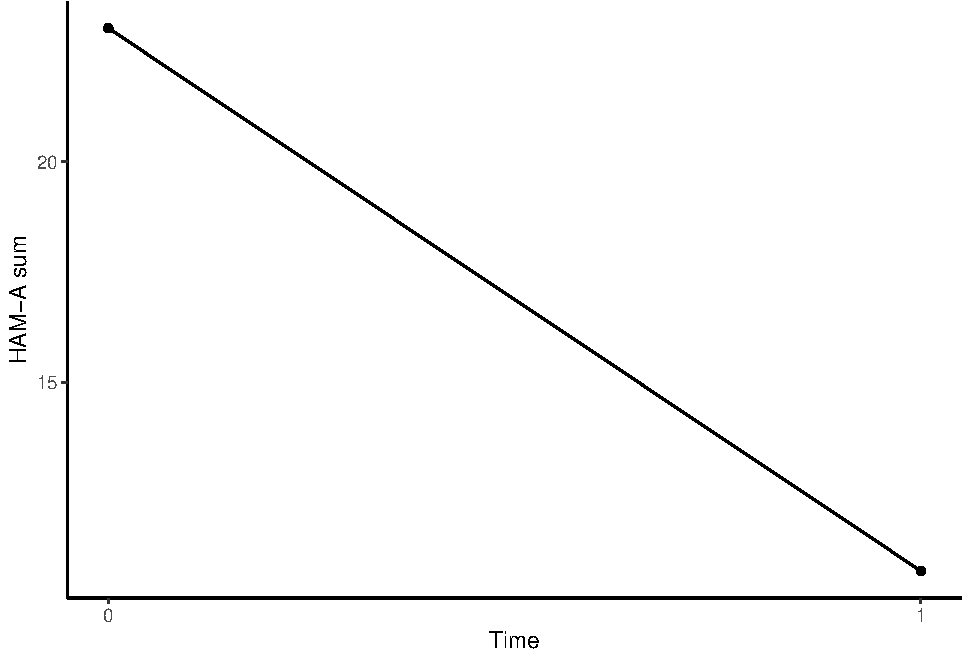
\includegraphics{DZP_R_bookdown_files/figure-latex/unnamed-chunk-10-1.pdf}

Analyze using LMM:

\begin{Shaded}
\begin{Highlighting}[]
\FunctionTok{summary}\NormalTok{(}\FunctionTok{lmer}\NormalTok{(sum }\SpecialCharTok{\textasciitilde{}}\NormalTok{ time }\SpecialCharTok{+}\NormalTok{ (}\DecValTok{1}\SpecialCharTok{|}\NormalTok{id), }\AttributeTok{data =}\NormalTok{ data\_cluster))}
\end{Highlighting}
\end{Shaded}

\begin{verbatim}
## boundary (singular) fit: see ?isSingular
\end{verbatim}

\begin{verbatim}
## Linear mixed model fit by REML. t-tests use Satterthwaite's method [
## lmerModLmerTest]
## Formula: sum ~ time + (1 | id)
##    Data: data_cluster
## 
## REML criterion at convergence: 4275.9
## 
## Scaled residuals: 
##     Min      1Q  Median      3Q     Max 
## -3.4157 -0.6507 -0.0258  0.6965  3.2589 
## 
## Random effects:
##  Groups   Name        Variance  Std.Dev. 
##  id       (Intercept) 5.860e-16 2.421e-08
##  Residual             2.635e+01 5.133e+00
## Number of obs: 700, groups:  id, 350
## 
## Fixed effects:
##             Estimate Std. Error       df t value Pr(>|t|)    
## (Intercept)  23.0323     0.2744 698.0000   83.95   <2e-16 ***
## time        -12.3096     0.3880 698.0000  -31.73   <2e-16 ***
## ---
## Signif. codes:  0 '***' 0.001 '**' 0.01 '*' 0.05 '.' 0.1 ' ' 1
## 
## Correlation of Fixed Effects:
##      (Intr)
## time -0.707
## optimizer (nloptwrap) convergence code: 0 (OK)
## boundary (singular) fit: see ?isSingular
\end{verbatim}

\hypertarget{prepare-for-clustering}{%
\subsection{Prepare for Clustering}\label{prepare-for-clustering}}

Let us see if we can find some item clusters in the baseline data to get a more differentiated picture:

For this we first need to drop the id, sum, and time columns:

\begin{Shaded}
\begin{Highlighting}[]
\NormalTok{data\_cluster\_bl }\OtherTok{=}\NormalTok{ BBmisc}\SpecialCharTok{::}\FunctionTok{dropNamed}\NormalTok{(data\_cluster\_bl, }\AttributeTok{drop =} \FunctionTok{c}\NormalTok{(}\StringTok{"time"}\NormalTok{, }\StringTok{"id"}\NormalTok{, }\StringTok{"sum"}\NormalTok{))}
\NormalTok{data\_cluster\_post }\OtherTok{=}\NormalTok{ BBmisc}\SpecialCharTok{::}\FunctionTok{dropNamed}\NormalTok{(data\_cluster\_post, }\AttributeTok{drop =} \FunctionTok{c}\NormalTok{(}\StringTok{"time"}\NormalTok{, }\StringTok{"id"}\NormalTok{, }\StringTok{"sum"}\NormalTok{))}
\end{Highlighting}
\end{Shaded}

As a first step, it makes sense to scale the data, as not all item formats are identical in all scales:

\begin{Shaded}
\begin{Highlighting}[]
\NormalTok{data\_cluster\_bl\_s }\OtherTok{=} \FunctionTok{scale}\NormalTok{(data\_cluster\_bl)}
\end{Highlighting}
\end{Shaded}

Next, we will transpose the data, since we want to cluster items into people and not vice versa:

\begin{Shaded}
\begin{Highlighting}[]
\NormalTok{data\_transposed }\OtherTok{=} \FunctionTok{t}\NormalTok{(}\FunctionTok{na.omit}\NormalTok{(data\_cluster\_bl\_s))}
\end{Highlighting}
\end{Shaded}

Now we will creat a distance matrix to determine the proximity between item responses. The euclidean distance is a commonly used measure for psychometric measures (another one is the manhattan distance).

\begin{Shaded}
\begin{Highlighting}[]
\NormalTok{d }\OtherTok{=} \FunctionTok{dist}\NormalTok{(data\_transposed, }\AttributeTok{method =} \StringTok{"euclidean"}\NormalTok{)}
\end{Highlighting}
\end{Shaded}

And now, let us cluster the data. We use the \texttt{ward.D2} method, this way distances are squared ahead of clustering (no problem with negative data):

\begin{Shaded}
\begin{Highlighting}[]
\NormalTok{clust }\OtherTok{=} \FunctionTok{hclust}\NormalTok{(d, }\AttributeTok{method =} \StringTok{"ward.D2"}\NormalTok{)}
\end{Highlighting}
\end{Shaded}

After the clustering is finished we should inspect the result. A common way to look at clustering solutions is the dendrogram:

\begin{Shaded}
\begin{Highlighting}[]
\NormalTok{dend }\OtherTok{\textless{}{-}} \FunctionTok{as.dendrogram}\NormalTok{(clust, }\AttributeTok{hang =} \SpecialCharTok{{-}}\DecValTok{1}\NormalTok{)}

\FunctionTok{labels\_cex}\NormalTok{(dend) }\OtherTok{=} \DecValTok{2}
\NormalTok{marg }\OtherTok{=} \FunctionTok{c}\NormalTok{(}\DecValTok{4}\NormalTok{, }\DecValTok{4}\NormalTok{, }\DecValTok{10}\NormalTok{, }\DecValTok{35}\NormalTok{)}
\FunctionTok{par}\NormalTok{(}\AttributeTok{mar =}\NormalTok{ marg, }\AttributeTok{font =} \DecValTok{1}\NormalTok{, }\AttributeTok{cex =} \FloatTok{0.4}\NormalTok{, }\AttributeTok{cex.axis =} \FloatTok{1.7}\NormalTok{, }\AttributeTok{cex.lab =} \DecValTok{2}\NormalTok{)}
\FunctionTok{plot}\NormalTok{(}\FunctionTok{rev}\NormalTok{(dend), }\AttributeTok{horiz =}\NormalTok{ T, }\AttributeTok{edgePar =} \FunctionTok{list}\NormalTok{(}\AttributeTok{lwd =} \DecValTok{2}\NormalTok{))}
\end{Highlighting}
\end{Shaded}

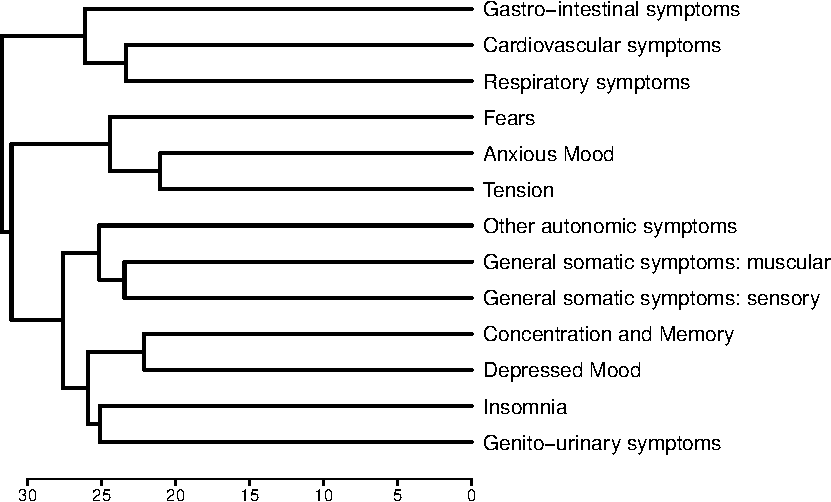
\includegraphics{DZP_R_bookdown_files/figure-latex/unnamed-chunk-17-1.pdf}

The earlier two items merge in the dendrogram, the more similar they were scored by the patients. We now have a good idea, which items belong together. However, now we need to decide how many clusters to retain, i.e.~where to ``cut'' our dendrogram. This step is called pruning.

We will use the \texttt{cutreeDynamic()} function from the \texttt{dynamicTreeCut} package. It has many advantages over traditional methods (e.g.~gap statistic, silhouette method) including that it is more sensitive for detection of distinct classes and more stable in bootstrapping procedures.

The argument \texttt{minClusterSize} should be set to 1 and the method should be \texttt{"hybrid"}.

\begin{Shaded}
\begin{Highlighting}[]
\NormalTok{pruned }\OtherTok{=}\NormalTok{ dynamicTreeCut}\SpecialCharTok{::}\FunctionTok{cutreeDynamic}\NormalTok{(clust, }\AttributeTok{distM =} \FunctionTok{as.matrix}\NormalTok{(d), }\AttributeTok{method =} \StringTok{"hybrid"}\NormalTok{, }\AttributeTok{minClusterSize =} \DecValTok{1}\NormalTok{)}
\end{Highlighting}
\end{Shaded}

\begin{verbatim}
##  ..cutHeight not given, setting it to 31.6  ===>  99% of the (truncated) height range in dendro.
##  ..done.
\end{verbatim}

\begin{Shaded}
\begin{Highlighting}[]
\NormalTok{pruned}
\end{Highlighting}
\end{Shaded}

\begin{verbatim}
## 1 1 1 2 2 2 4 4 3 3 3 2 4 
## 2 2 2 1 1 1 4 4 3 3 3 1 4
\end{verbatim}

The \texttt{pruned} object includes our final clustering solution (i.e.~which item belongs to which cluster).

We should pass the same names to it, that we used for the items:

\begin{Shaded}
\begin{Highlighting}[]
\FunctionTok{names}\NormalTok{(pruned) }\OtherTok{=}\NormalTok{ hama\_names}
\NormalTok{pruned}
\end{Highlighting}
\end{Shaded}

\begin{verbatim}
##                       Anxious Mood                            Tension 
##                                  2                                  2 
##                              Fears                           Insomnia 
##                                  2                                  1 
##           Concentration and Memory                     Depressed Mood 
##                                  1                                  1 
## General somatic symptoms: muscular  General somatic symptoms: sensory 
##                                  4                                  4 
##            Cardiovascular symptoms               Respiratory symptoms 
##                                  3                                  3 
##         Gastro-intestinal symptoms            Genito-urinary symptoms 
##                                  3                                  1 
##           Other autonomic symptoms 
##                                  4
\end{verbatim}

Now we can plot our pruned dendrogram. We will indicate class membership using colours:

\begin{Shaded}
\begin{Highlighting}[]
\FunctionTok{labels\_colors}\NormalTok{(dend) }\OtherTok{=}\NormalTok{ pruned[}\FunctionTok{c}\NormalTok{(clust}\SpecialCharTok{$}\NormalTok{order)]}
\FunctionTok{labels\_cex}\NormalTok{(dend) }\OtherTok{=} \DecValTok{2}
\NormalTok{marg }\OtherTok{=} \FunctionTok{c}\NormalTok{(}\DecValTok{4}\NormalTok{, }\DecValTok{4}\NormalTok{, }\DecValTok{10}\NormalTok{, }\DecValTok{35}\NormalTok{)}
\FunctionTok{par}\NormalTok{(}\AttributeTok{mar =}\NormalTok{ marg, }\AttributeTok{font =} \DecValTok{1}\NormalTok{, }\AttributeTok{cex =} \FloatTok{0.4}\NormalTok{, }\AttributeTok{cex.axis =} \FloatTok{1.7}\NormalTok{, }\AttributeTok{cex.lab =} \DecValTok{2}\NormalTok{)}
\FunctionTok{plot}\NormalTok{(}\FunctionTok{rev}\NormalTok{(dend), }\AttributeTok{horiz =}\NormalTok{ T, }\AttributeTok{edgePar =} \FunctionTok{list}\NormalTok{(}\AttributeTok{lwd =} \DecValTok{2}\NormalTok{))}
\end{Highlighting}
\end{Shaded}

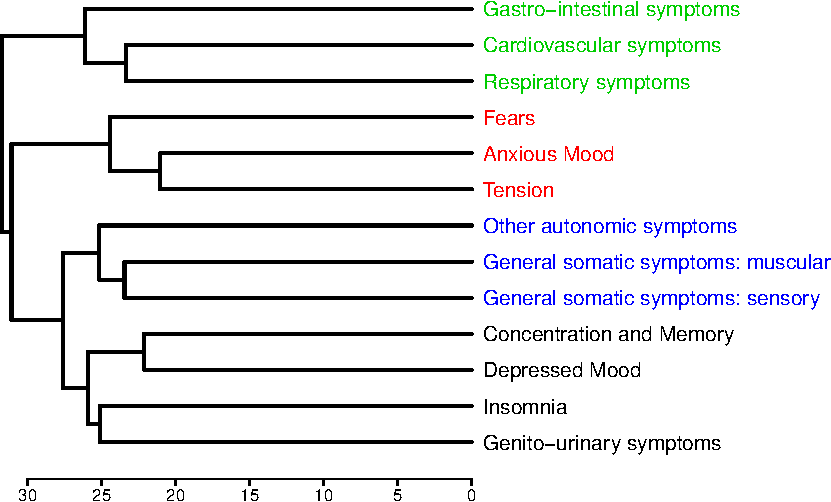
\includegraphics{DZP_R_bookdown_files/figure-latex/unnamed-chunk-20-1.pdf}

\begin{Shaded}
\begin{Highlighting}[]
\NormalTok{data\_cluster\_bl}\SpecialCharTok{$}\NormalTok{id }\OtherTok{=} \FunctionTok{row.names}\NormalTok{(data\_cluster\_bl)}
\NormalTok{data\_cluster\_bl}\SpecialCharTok{$}\NormalTok{time }\OtherTok{=} \DecValTok{0}
\NormalTok{data\_cluster\_post}\SpecialCharTok{$}\NormalTok{id }\OtherTok{=} \FunctionTok{row.names}\NormalTok{(data\_cluster\_post)}
\NormalTok{data\_cluster\_post}\SpecialCharTok{$}\NormalTok{time }\OtherTok{=} \DecValTok{1}
\end{Highlighting}
\end{Shaded}

\begin{Shaded}
\begin{Highlighting}[]
\NormalTok{data\_cluster\_bl}\SpecialCharTok{$}\NormalTok{sum\_c1 }\OtherTok{=} \FunctionTok{rowSums}\NormalTok{(data\_cluster\_bl[}\FunctionTok{which}\NormalTok{(pruned }\SpecialCharTok{==} \DecValTok{1}\NormalTok{)]) }\SpecialCharTok{/} \FunctionTok{length}\NormalTok{(}\FunctionTok{which}\NormalTok{(pruned }\SpecialCharTok{==} \DecValTok{1}\NormalTok{))}
\NormalTok{data\_cluster\_bl}\SpecialCharTok{$}\NormalTok{sum\_c2 }\OtherTok{=} \FunctionTok{rowSums}\NormalTok{(data\_cluster\_bl[}\FunctionTok{which}\NormalTok{(pruned }\SpecialCharTok{==} \DecValTok{2}\NormalTok{)]) }\SpecialCharTok{/} \FunctionTok{length}\NormalTok{(}\FunctionTok{which}\NormalTok{(pruned }\SpecialCharTok{==} \DecValTok{2}\NormalTok{))}
\NormalTok{data\_cluster\_bl}\SpecialCharTok{$}\NormalTok{sum\_c3 }\OtherTok{=} \FunctionTok{rowSums}\NormalTok{(data\_cluster\_bl[}\FunctionTok{which}\NormalTok{(pruned }\SpecialCharTok{==} \DecValTok{3}\NormalTok{)]) }\SpecialCharTok{/} \FunctionTok{length}\NormalTok{(}\FunctionTok{which}\NormalTok{(pruned }\SpecialCharTok{==} \DecValTok{3}\NormalTok{))}
\NormalTok{data\_cluster\_bl}\SpecialCharTok{$}\NormalTok{sum\_c4 }\OtherTok{=} \FunctionTok{rowSums}\NormalTok{(data\_cluster\_bl[}\FunctionTok{which}\NormalTok{(pruned }\SpecialCharTok{==} \DecValTok{4}\NormalTok{)]) }\SpecialCharTok{/} \FunctionTok{length}\NormalTok{(}\FunctionTok{which}\NormalTok{(pruned }\SpecialCharTok{==} \DecValTok{4}\NormalTok{))}

\NormalTok{data\_cluster\_post}\SpecialCharTok{$}\NormalTok{sum\_c1 }\OtherTok{=} \FunctionTok{rowSums}\NormalTok{(data\_cluster\_post[}\FunctionTok{which}\NormalTok{(pruned }\SpecialCharTok{==} \DecValTok{1}\NormalTok{)]) }\SpecialCharTok{/} \FunctionTok{length}\NormalTok{(}\FunctionTok{which}\NormalTok{(pruned }\SpecialCharTok{==} \DecValTok{1}\NormalTok{))}
\NormalTok{data\_cluster\_post}\SpecialCharTok{$}\NormalTok{sum\_c2 }\OtherTok{=} \FunctionTok{rowSums}\NormalTok{(data\_cluster\_post[}\FunctionTok{which}\NormalTok{(pruned }\SpecialCharTok{==} \DecValTok{2}\NormalTok{)]) }\SpecialCharTok{/} \FunctionTok{length}\NormalTok{(}\FunctionTok{which}\NormalTok{(pruned }\SpecialCharTok{==} \DecValTok{1}\NormalTok{))}
\NormalTok{data\_cluster\_post}\SpecialCharTok{$}\NormalTok{sum\_c3 }\OtherTok{=} \FunctionTok{rowSums}\NormalTok{(data\_cluster\_post[}\FunctionTok{which}\NormalTok{(pruned }\SpecialCharTok{==} \DecValTok{3}\NormalTok{)]) }\SpecialCharTok{/} \FunctionTok{length}\NormalTok{(}\FunctionTok{which}\NormalTok{(pruned }\SpecialCharTok{==} \DecValTok{1}\NormalTok{))}
\NormalTok{data\_cluster\_post}\SpecialCharTok{$}\NormalTok{sum\_c4 }\OtherTok{=} \FunctionTok{rowSums}\NormalTok{(data\_cluster\_post[}\FunctionTok{which}\NormalTok{(pruned }\SpecialCharTok{==} \DecValTok{4}\NormalTok{)]) }\SpecialCharTok{/} \FunctionTok{length}\NormalTok{(}\FunctionTok{which}\NormalTok{(pruned }\SpecialCharTok{==} \DecValTok{1}\NormalTok{))}
\end{Highlighting}
\end{Shaded}

\begin{Shaded}
\begin{Highlighting}[]
\NormalTok{data\_cluster }\OtherTok{=} \FunctionTok{rbind}\NormalTok{(data\_cluster\_bl, data\_cluster\_post)}
\NormalTok{data\_cluster\_long }\OtherTok{=}\NormalTok{ multilevel}\SpecialCharTok{::}\FunctionTok{make.univ}\NormalTok{(data\_cluster, data\_cluster[,}\FunctionTok{grep}\NormalTok{(}\StringTok{"sum"}\NormalTok{, }\FunctionTok{names}\NormalTok{(data\_cluster))], }\AttributeTok{outname =} \StringTok{"Symptoms"}\NormalTok{)}
\NormalTok{data\_cluster\_long }\OtherTok{=} \FunctionTok{rename}\NormalTok{(data\_cluster\_long, }\AttributeTok{Cluster =}\NormalTok{ TIME)}
\NormalTok{data\_cluster\_long}\SpecialCharTok{$}\NormalTok{Cluster }\OtherTok{=}\NormalTok{ data\_cluster\_long}\SpecialCharTok{$}\NormalTok{Cluster }\SpecialCharTok{+}\DecValTok{1}
\NormalTok{data\_cluster\_long}\SpecialCharTok{$}\NormalTok{Cluster }\OtherTok{=} \FunctionTok{factor}\NormalTok{(data\_cluster\_long}\SpecialCharTok{$}\NormalTok{Cluster)}
\end{Highlighting}
\end{Shaded}

\begin{Shaded}
\begin{Highlighting}[]
\FunctionTok{ggplot}\NormalTok{(}\AttributeTok{data =}\NormalTok{ data\_cluster\_long, }\FunctionTok{aes}\NormalTok{(}\AttributeTok{x =}\NormalTok{ time, }\AttributeTok{y =}\NormalTok{ Symptoms, }\AttributeTok{colour =}\NormalTok{ Cluster)) }\SpecialCharTok{+}
  \FunctionTok{stat\_summary}\NormalTok{(}\AttributeTok{geom =} \StringTok{"line"}\NormalTok{, }\AttributeTok{fun =} \StringTok{"mean"}\NormalTok{) }\SpecialCharTok{+}
   \FunctionTok{stat\_summary}\NormalTok{(}\AttributeTok{geom =} \StringTok{"point"}\NormalTok{, }\AttributeTok{fun =} \StringTok{"mean"}\NormalTok{) }\SpecialCharTok{+}
  \FunctionTok{scale\_x\_continuous}\NormalTok{(}\AttributeTok{breaks =} \FunctionTok{c}\NormalTok{(}\DecValTok{0}\NormalTok{,}\DecValTok{1}\NormalTok{)) }\SpecialCharTok{+}
  \FunctionTok{labs}\NormalTok{(}\AttributeTok{y =} \StringTok{"Clusterscore"}\NormalTok{, }\AttributeTok{x =} \StringTok{"Time"}\NormalTok{) }\SpecialCharTok{+}
  \FunctionTok{theme\_classic}\NormalTok{()}
\end{Highlighting}
\end{Shaded}

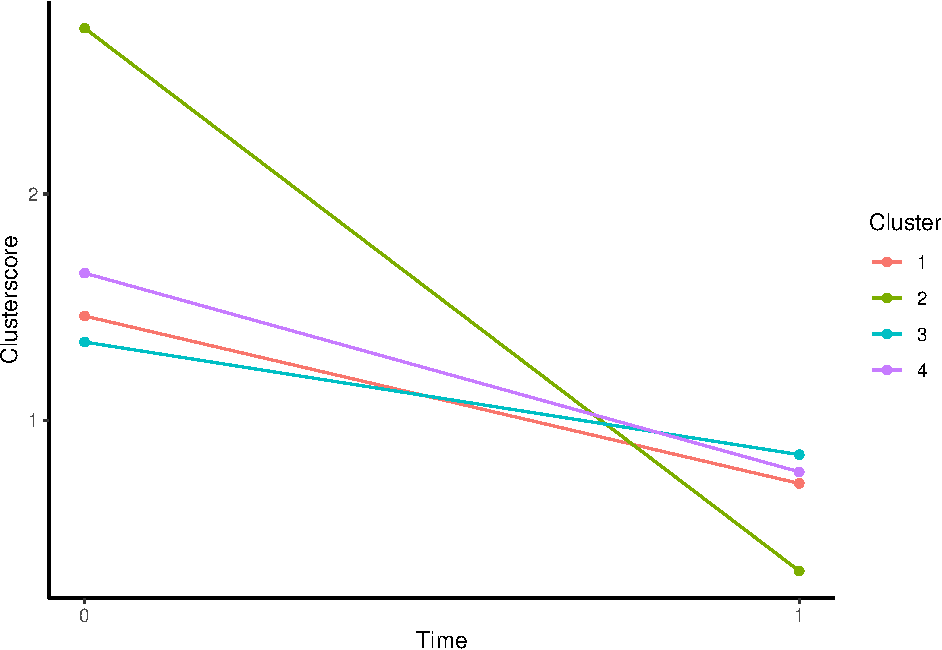
\includegraphics{DZP_R_bookdown_files/figure-latex/unnamed-chunk-24-1.pdf}

Let us model change, but now as a function of cluster:

First let us check the omnibus test:

\begin{Shaded}
\begin{Highlighting}[]
\NormalTok{mod }\OtherTok{=} \FunctionTok{lmer}\NormalTok{(Symptoms }\SpecialCharTok{\textasciitilde{}}\NormalTok{ time }\SpecialCharTok{*}\NormalTok{ Cluster }\SpecialCharTok{+}\NormalTok{ (}\DecValTok{1}\SpecialCharTok{|}\NormalTok{id), }\AttributeTok{data =}\NormalTok{ data\_cluster\_long)}

\FunctionTok{anova}\NormalTok{(mod)}
\end{Highlighting}
\end{Shaded}

\begin{verbatim}
## Type III Analysis of Variance Table with Satterthwaite's method
##              Sum Sq Mean Sq NumDF DenDF F value    Pr(>F)    
## time         889.75  889.75     1  2443 1963.83 < 2.2e-16 ***
## Cluster      424.03  141.34     3  2443  311.97 < 2.2e-16 ***
## time:Cluster 388.60  129.53     3  2443  285.90 < 2.2e-16 ***
## ---
## Signif. codes:  0 '***' 0.001 '**' 0.01 '*' 0.05 '.' 0.1 ' ' 1
\end{verbatim}

There is a significant Cluster x Time interaction. Let us probe the interaction effect using pairwise comparisons between the cluster-specific slopes:

\begin{Shaded}
\begin{Highlighting}[]
\NormalTok{emmeans}\SpecialCharTok{::}\FunctionTok{emtrends}\NormalTok{(mod, }\AttributeTok{specs =}\NormalTok{ pairwise }\SpecialCharTok{\textasciitilde{}}\NormalTok{ Cluster, }\AttributeTok{var =} \StringTok{"time"}\NormalTok{)}
\end{Highlighting}
\end{Shaded}

\begin{verbatim}
## $emtrends
##  Cluster time.trend     SE   df lower.CL upper.CL
##  1           -0.739 0.0509 2443   -0.839   -0.639
##  2           -2.396 0.0509 2443   -2.496   -2.296
##  3           -0.497 0.0509 2443   -0.597   -0.397
##  4           -0.877 0.0509 2443   -0.977   -0.777
## 
## Results are averaged over the levels of: time 
## Degrees-of-freedom method: kenward-roger 
## Confidence level used: 0.95 
## 
## $contrasts
##  contrast            estimate    SE   df t.ratio p.value
##  Cluster1 - Cluster2    1.657 0.072 2443  23.029  <.0001
##  Cluster1 - Cluster3   -0.242 0.072 2443  -3.363  0.0043
##  Cluster1 - Cluster4    0.138 0.072 2443   1.920  0.2197
##  Cluster2 - Cluster3   -1.899 0.072 2443 -26.392  <.0001
##  Cluster2 - Cluster4   -1.519 0.072 2443 -21.109  <.0001
##  Cluster3 - Cluster4    0.380 0.072 2443   5.283  <.0001
## 
## Results are averaged over the levels of: time 
## Degrees-of-freedom method: kenward-roger 
## P value adjustment: tukey method for comparing a family of 4 estimates
\end{verbatim}

\hypertarget{exercise-2-response-trajectories}{%
\section{Exercise 2: Response Trajectories}\label{exercise-2-response-trajectories}}

\hypertarget{simulate-practice-data-1}{%
\subsection{Simulate Practice Data}\label{simulate-practice-data-1}}

\begin{Shaded}
\begin{Highlighting}[]
\NormalTok{n }\OtherTok{=} \DecValTok{350} \CommentTok{\# number of individuals}
\NormalTok{t }\OtherTok{=} \DecValTok{1}\SpecialCharTok{:}\DecValTok{10}   \CommentTok{\# number of time periods}

\NormalTok{df }\OtherTok{=} \FunctionTok{expand.grid}\NormalTok{(}\AttributeTok{t =} \DecValTok{1}\SpecialCharTok{:}\FunctionTok{max}\NormalTok{(t),}
                 \AttributeTok{id =} \DecValTok{1}\SpecialCharTok{:}\NormalTok{n)}
\NormalTok{df}\SpecialCharTok{$}\NormalTok{group }\OtherTok{=} \FunctionTok{c}\NormalTok{(}\FunctionTok{rep}\NormalTok{(}\StringTok{"active"}\NormalTok{, }\FunctionTok{nrow}\NormalTok{(df)}\SpecialCharTok{/}\DecValTok{2}\NormalTok{), }\FunctionTok{rep}\NormalTok{(}\StringTok{"placebo"}\NormalTok{, }\FunctionTok{nrow}\NormalTok{(df)}\SpecialCharTok{/}\DecValTok{2}\NormalTok{))}

\NormalTok{trajectory }\OtherTok{=} \FunctionTok{c}\NormalTok{(}\StringTok{"Linear response"}\NormalTok{,}
               \StringTok{"Deteriorate"}\NormalTok{,}
               \StringTok{"Rev. U{-}shape"}\NormalTok{,}
               \StringTok{"Rapid response"}\NormalTok{,}
               \StringTok{"No change"}\NormalTok{)}

\FunctionTok{set.seed}\NormalTok{(}\DecValTok{123}\NormalTok{)}
\ControlFlowTok{for}\NormalTok{(ch }\ControlFlowTok{in} \FunctionTok{unique}\NormalTok{(df}\SpecialCharTok{$}\NormalTok{id))\{}

  \ControlFlowTok{if}\NormalTok{(df}\SpecialCharTok{$}\NormalTok{group[df}\SpecialCharTok{$}\NormalTok{id }\SpecialCharTok{==}\NormalTok{ ch][}\DecValTok{1}\NormalTok{] }\SpecialCharTok{==} \StringTok{"active"}\NormalTok{)\{}
\NormalTok{    df}\SpecialCharTok{$}\NormalTok{trajectory[df}\SpecialCharTok{$}\NormalTok{id }\SpecialCharTok{==}\NormalTok{ ch] }\OtherTok{=} \FunctionTok{rep}\NormalTok{(}\FunctionTok{sample}\NormalTok{(trajectory, }\AttributeTok{size =} \DecValTok{1}\NormalTok{, }\AttributeTok{replace =}\NormalTok{ T, }\AttributeTok{prob =} \FunctionTok{c}\NormalTok{(.}\DecValTok{5}\NormalTok{, .}\DecValTok{05}\NormalTok{, .}\DecValTok{2}\NormalTok{, .}\DecValTok{2}\NormalTok{, .}\DecValTok{05}\NormalTok{)), }\FunctionTok{max}\NormalTok{(t))}
\NormalTok{  \}}
  \ControlFlowTok{if}\NormalTok{(df}\SpecialCharTok{$}\NormalTok{group[df}\SpecialCharTok{$}\NormalTok{id }\SpecialCharTok{==}\NormalTok{ ch][}\DecValTok{1}\NormalTok{] }\SpecialCharTok{==} \StringTok{"placebo"}\NormalTok{)\{}
\NormalTok{    df}\SpecialCharTok{$}\NormalTok{trajectory[df}\SpecialCharTok{$}\NormalTok{id }\SpecialCharTok{==}\NormalTok{ ch] }\OtherTok{=} \FunctionTok{rep}\NormalTok{(}\FunctionTok{sample}\NormalTok{(trajectory, }\AttributeTok{size =} \DecValTok{1}\NormalTok{, }\AttributeTok{replace =}\NormalTok{ T, }\AttributeTok{prob =} \FunctionTok{c}\NormalTok{(.}\DecValTok{2}\NormalTok{, .}\DecValTok{2}\NormalTok{, .}\DecValTok{1}\NormalTok{, .}\DecValTok{05}\NormalTok{, .}\DecValTok{45}\NormalTok{)), }\FunctionTok{max}\NormalTok{(t))}
\NormalTok{  \}}

  \ControlFlowTok{if}\NormalTok{(df}\SpecialCharTok{$}\NormalTok{trajectory[df}\SpecialCharTok{$}\NormalTok{id }\SpecialCharTok{==}\NormalTok{ ch][}\DecValTok{1}\NormalTok{] }\SpecialCharTok{==} \StringTok{"No change"}\NormalTok{)\{}
\NormalTok{    df}\SpecialCharTok{$}\NormalTok{y[df}\SpecialCharTok{$}\NormalTok{id }\SpecialCharTok{==}\NormalTok{ ch] }\OtherTok{=} \DecValTok{24} \SpecialCharTok{+} \DecValTok{0}\SpecialCharTok{*}\NormalTok{t  }\SpecialCharTok{+} \FunctionTok{rnorm}\NormalTok{(}\FunctionTok{nrow}\NormalTok{(df[df}\SpecialCharTok{$}\NormalTok{id }\SpecialCharTok{==}\NormalTok{ ch,]), }\DecValTok{0}\NormalTok{, }\DecValTok{3}\NormalTok{)}
\NormalTok{  \}}
  \ControlFlowTok{if}\NormalTok{(df}\SpecialCharTok{$}\NormalTok{trajectory[df}\SpecialCharTok{$}\NormalTok{id }\SpecialCharTok{==}\NormalTok{ ch][}\DecValTok{1}\NormalTok{] }\SpecialCharTok{==} \StringTok{"Rev. U{-}shape"}\NormalTok{)\{}
\NormalTok{    df}\SpecialCharTok{$}\NormalTok{y[df}\SpecialCharTok{$}\NormalTok{id }\SpecialCharTok{==}\NormalTok{ ch] }\OtherTok{=} \DecValTok{24} \SpecialCharTok{+} \DecValTok{8}\SpecialCharTok{*}\NormalTok{t }\SpecialCharTok{{-}} \FloatTok{0.9}\SpecialCharTok{*}\NormalTok{t}\SpecialCharTok{\^{}}\DecValTok{2} \SpecialCharTok{+} \FunctionTok{rnorm}\NormalTok{(}\FunctionTok{nrow}\NormalTok{(df[df}\SpecialCharTok{$}\NormalTok{id }\SpecialCharTok{==}\NormalTok{ ch,]), }\DecValTok{0}\NormalTok{, }\DecValTok{3}\NormalTok{)}
\NormalTok{  \}}
  \ControlFlowTok{if}\NormalTok{(df}\SpecialCharTok{$}\NormalTok{trajectory[df}\SpecialCharTok{$}\NormalTok{id }\SpecialCharTok{==}\NormalTok{ ch][}\DecValTok{1}\NormalTok{] }\SpecialCharTok{==} \StringTok{"Linear response"}\NormalTok{)\{}
\NormalTok{    df}\SpecialCharTok{$}\NormalTok{y[df}\SpecialCharTok{$}\NormalTok{id }\SpecialCharTok{==}\NormalTok{ ch] }\OtherTok{=} \DecValTok{24} \SpecialCharTok{{-}} \DecValTok{1}\SpecialCharTok{*}\NormalTok{t  }\SpecialCharTok{+} \FunctionTok{rnorm}\NormalTok{(}\FunctionTok{nrow}\NormalTok{(df[df}\SpecialCharTok{$}\NormalTok{id }\SpecialCharTok{==}\NormalTok{ ch,]), }\DecValTok{0}\NormalTok{, }\DecValTok{3}\NormalTok{)}
\NormalTok{  \}}
  \ControlFlowTok{if}\NormalTok{(df}\SpecialCharTok{$}\NormalTok{trajectory[df}\SpecialCharTok{$}\NormalTok{id }\SpecialCharTok{==}\NormalTok{ ch][}\DecValTok{1}\NormalTok{] }\SpecialCharTok{==} \StringTok{"Deteriorate"}\NormalTok{)\{}
\NormalTok{    df}\SpecialCharTok{$}\NormalTok{y[df}\SpecialCharTok{$}\NormalTok{id }\SpecialCharTok{==}\NormalTok{ ch] }\OtherTok{=} \DecValTok{24} \SpecialCharTok{+} \DecValTok{2}\SpecialCharTok{*}\NormalTok{t  }\SpecialCharTok{+} \FunctionTok{rnorm}\NormalTok{(}\FunctionTok{nrow}\NormalTok{(df[df}\SpecialCharTok{$}\NormalTok{id }\SpecialCharTok{==}\NormalTok{ ch,]), }\DecValTok{0}\NormalTok{, }\DecValTok{3}\NormalTok{)}
\NormalTok{  \}}
  \ControlFlowTok{if}\NormalTok{(df}\SpecialCharTok{$}\NormalTok{trajectory[df}\SpecialCharTok{$}\NormalTok{id }\SpecialCharTok{==}\NormalTok{ ch][}\DecValTok{1}\NormalTok{] }\SpecialCharTok{==} \StringTok{"Rapid response"}\NormalTok{)\{}
\NormalTok{    df}\SpecialCharTok{$}\NormalTok{y[df}\SpecialCharTok{$}\NormalTok{id }\SpecialCharTok{==}\NormalTok{ ch] }\OtherTok{=} \DecValTok{24} \SpecialCharTok{{-}} \DecValTok{10} \SpecialCharTok{*} \FunctionTok{log}\NormalTok{(t) }\SpecialCharTok{+}  \FunctionTok{rnorm}\NormalTok{(}\FunctionTok{nrow}\NormalTok{(df[df}\SpecialCharTok{$}\NormalTok{id }\SpecialCharTok{==}\NormalTok{ ch,]), }\DecValTok{0}\NormalTok{, }\DecValTok{3}\NormalTok{)}
\NormalTok{  \}}
\NormalTok{\}}
\end{Highlighting}
\end{Shaded}

\hypertarget{inspect-the-data}{%
\subsection{Inspect the Data}\label{inspect-the-data}}

Plot the data as we usually would (one trajectory per group)

\begin{Shaded}
\begin{Highlighting}[]
\FunctionTok{ggplot}\NormalTok{(}\AttributeTok{data =}\NormalTok{ df, }\FunctionTok{aes}\NormalTok{(}\AttributeTok{x =}\NormalTok{ t, }\AttributeTok{y =}\NormalTok{ y, }\AttributeTok{colour =}\NormalTok{ group)) }\SpecialCharTok{+}
  \FunctionTok{stat\_summary}\NormalTok{(}\AttributeTok{geom =} \StringTok{"line"}\NormalTok{, }\AttributeTok{fun =} \StringTok{"mean"}\NormalTok{) }\SpecialCharTok{+}
  \FunctionTok{stat\_summary}\NormalTok{(}\AttributeTok{geom =} \StringTok{"point"}\NormalTok{, }\AttributeTok{fun =} \StringTok{"mean"}\NormalTok{) }\SpecialCharTok{+}
  \FunctionTok{scale\_x\_continuous}\NormalTok{(}\AttributeTok{breaks =}\NormalTok{ t) }\SpecialCharTok{+}
  \FunctionTok{coord\_cartesian}\NormalTok{(}\AttributeTok{ylim =} \FunctionTok{c}\NormalTok{(}\DecValTok{0}\NormalTok{,}\DecValTok{50}\NormalTok{)) }\SpecialCharTok{+}
  \FunctionTok{labs}\NormalTok{(}\AttributeTok{x =} \StringTok{"Time"}\NormalTok{, }\AttributeTok{colour =} \StringTok{"Group"}\NormalTok{) }\SpecialCharTok{+}
  \FunctionTok{theme\_classic}\NormalTok{()}
\end{Highlighting}
\end{Shaded}

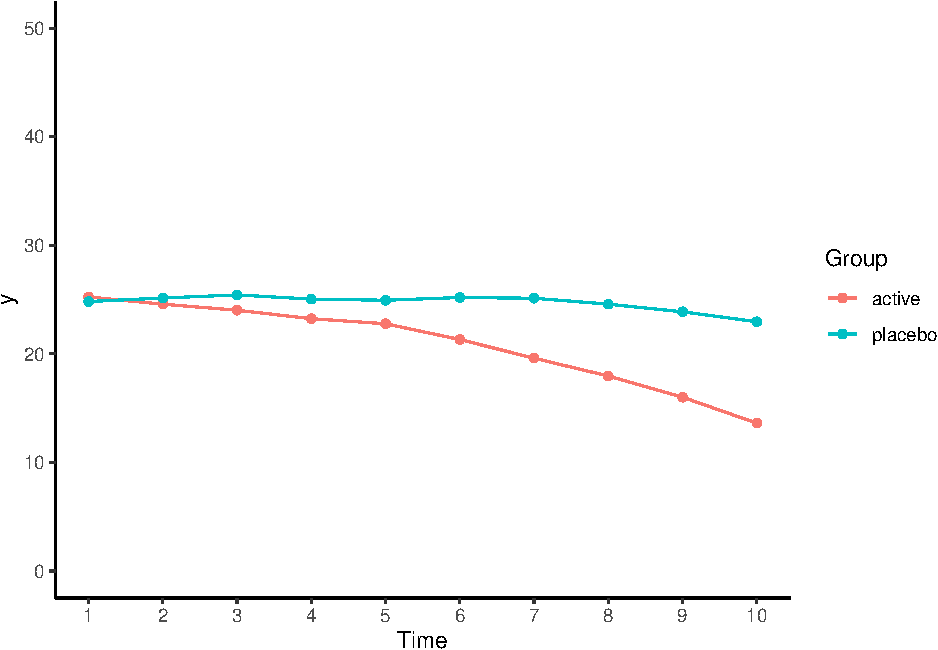
\includegraphics{DZP_R_bookdown_files/figure-latex/unnamed-chunk-28-1.pdf}

Analyze using linear mixed model:

\begin{Shaded}
\begin{Highlighting}[]
\FunctionTok{library}\NormalTok{(lme4)}
\FunctionTok{library}\NormalTok{(lmerTest)}

\FunctionTok{summary}\NormalTok{(}\FunctionTok{lmer}\NormalTok{(y }\SpecialCharTok{\textasciitilde{}}\NormalTok{ t }\SpecialCharTok{*}\NormalTok{ group }\SpecialCharTok{+}\NormalTok{ (}\DecValTok{1}\SpecialCharTok{|}\NormalTok{id), }\AttributeTok{data =}\NormalTok{ df))}
\end{Highlighting}
\end{Shaded}

\begin{verbatim}
## Linear mixed model fit by REML. t-tests use Satterthwaite's method [
## lmerModLmerTest]
## Formula: y ~ t * group + (1 | id)
##    Data: df
## 
## REML criterion at convergence: 22778.7
## 
## Scaled residuals: 
##     Min      1Q  Median      3Q     Max 
## -4.4769 -0.5261 -0.0116  0.5401  3.7271 
## 
## Random effects:
##  Groups   Name        Variance Std.Dev.
##  id       (Intercept) 61.64    7.851   
##  Residual             28.74    5.361   
## Number of obs: 3500, groups:  id, 350
## 
## Fixed effects:
##                  Estimate Std. Error         df t value Pr(>|t|)    
## (Intercept)      27.73980    0.65488  469.59512  42.358   <2e-16 ***
## t                -1.25607    0.04462 3148.00004 -28.152   <2e-16 ***
## groupplacebo     -2.05383    0.92614  469.59513  -2.218   0.0271 *  
## t:groupplacebo    1.07806    0.06310 3148.00002  17.085   <2e-16 ***
## ---
## Signif. codes:  0 '***' 0.001 '**' 0.01 '*' 0.05 '.' 0.1 ' ' 1
## 
## Correlation of Fixed Effects:
##             (Intr) t      grpplc
## t           -0.375              
## groupplaceb -0.707  0.265       
## t:groupplcb  0.265 -0.707 -0.375
\end{verbatim}

Plot data on individual change groups (without the mixture model, we usually do not know these in advance):

\begin{Shaded}
\begin{Highlighting}[]
\FunctionTok{ggplot}\NormalTok{(}\AttributeTok{data =}\NormalTok{ df, }\FunctionTok{aes}\NormalTok{(}\AttributeTok{x =}\NormalTok{ t, }\AttributeTok{y =}\NormalTok{ y, }\AttributeTok{colour =}\NormalTok{ trajectory)) }\SpecialCharTok{+}
  \FunctionTok{geom\_point}\NormalTok{() }\SpecialCharTok{+}
  \FunctionTok{scale\_x\_continuous}\NormalTok{(}\AttributeTok{breaks =}\NormalTok{ t) }\SpecialCharTok{+}
  \FunctionTok{coord\_cartesian}\NormalTok{(}\AttributeTok{ylim =} \FunctionTok{c}\NormalTok{(}\DecValTok{0}\NormalTok{,}\DecValTok{50}\NormalTok{)) }\SpecialCharTok{+}
  \FunctionTok{facet\_grid}\NormalTok{(}\AttributeTok{cols =} \FunctionTok{vars}\NormalTok{(trajectory), }\AttributeTok{rows =} \FunctionTok{vars}\NormalTok{(group)) }\SpecialCharTok{+}
  \FunctionTok{labs}\NormalTok{(}\AttributeTok{colour =} \StringTok{"trajectory"}\NormalTok{, }\AttributeTok{x =} \StringTok{"Time"}\NormalTok{) }\SpecialCharTok{+}
  \FunctionTok{theme\_classic}\NormalTok{()}
\end{Highlighting}
\end{Shaded}

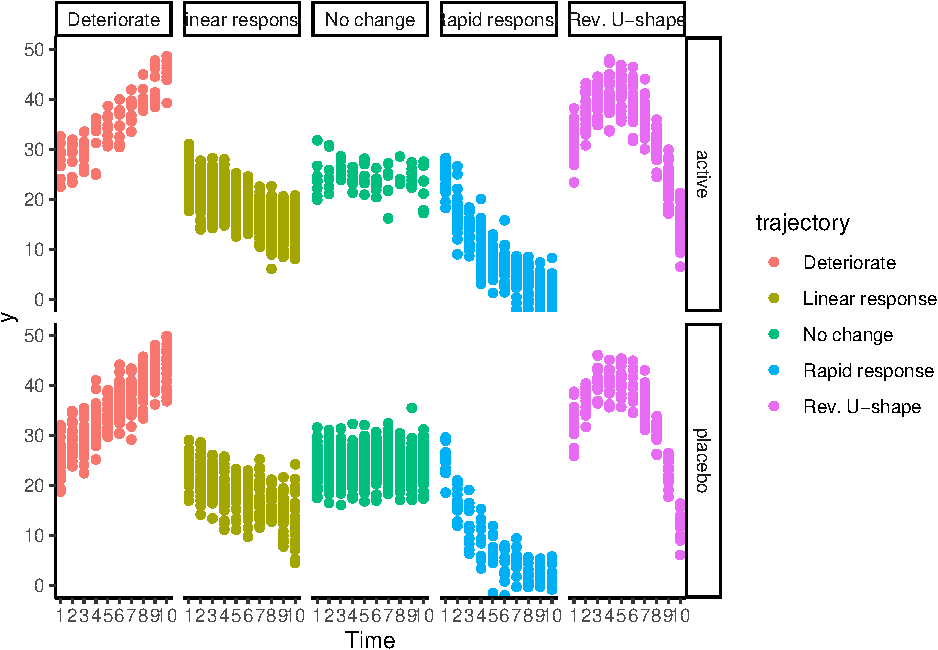
\includegraphics{DZP_R_bookdown_files/figure-latex/unnamed-chunk-30-1.pdf}

\hypertarget{create-lclmm}{%
\subsection{Create LCLMM}\label{create-lclmm}}

To identify reasonable grouping categories for these individually improving patients, we need to build a latent model.

Let us compute a growth mixtue model aka. latent class linear mixed models (LCLMM). We use the package \texttt{lcmm} for this.

\begin{itemize}
\item
  The \texttt{fixed} argument is a formula, as we know it from mixed models. We determine a polynomial here (usually quadratic or cubic as this is how most symptoms have been shown to change).
\item
  The \texttt{mixture} argument specifies class-specific fixed effects. These are the change parameters the trajectories are defined on
\item
  The \texttt{mixture} argument specifies a random argument as in the LMM. May be \texttt{\textasciitilde{}\ 1} for random intercepts or \texttt{1\ +\ t} for random intercepts and slopes.
\item
  The \texttt{ng} argument specifies the number of classes to be extracted. We will learn in a second how the optimal number of classes can be determined.
\item
  The \texttt{subject} argument specifies the nesting structure due to the repeated measurements.
\end{itemize}

\begin{Shaded}
\begin{Highlighting}[]
\FunctionTok{library}\NormalTok{(lcmm)}
\FunctionTok{library}\NormalTok{(LCTMtools)}

\NormalTok{mi }\OtherTok{=}\NormalTok{ lcmm}\SpecialCharTok{::}\FunctionTok{hlme}\NormalTok{(}\AttributeTok{fixed =}\NormalTok{ y }\SpecialCharTok{\textasciitilde{}} \DecValTok{1} \SpecialCharTok{+}\NormalTok{ t }\SpecialCharTok{+} \FunctionTok{I}\NormalTok{(t}\SpecialCharTok{\^{}}\DecValTok{2}\NormalTok{),}
           \AttributeTok{mixture =} \SpecialCharTok{\textasciitilde{}} \DecValTok{1} \SpecialCharTok{+}\NormalTok{ t }\SpecialCharTok{+} \FunctionTok{I}\NormalTok{(t}\SpecialCharTok{\^{}}\DecValTok{2}\NormalTok{),}
           \AttributeTok{random =} \SpecialCharTok{\textasciitilde{}} \DecValTok{1}\NormalTok{,}
           \AttributeTok{ng =} \DecValTok{5}\NormalTok{,}
           \AttributeTok{data =}\NormalTok{ df,}
           \AttributeTok{subject =} \StringTok{"id"}\NormalTok{)}
\end{Highlighting}
\end{Shaded}

\begin{verbatim}
## Be patient, hlme is running ... 
## The program took 7.48 seconds
\end{verbatim}

\hypertarget{inspect-the-lclmm-model}{%
\subsection{Inspect the LCLMM Model}\label{inspect-the-lclmm-model}}

Let us check the mixture object \texttt{mi}:

\begin{Shaded}
\begin{Highlighting}[]
\NormalTok{mi}
\end{Highlighting}
\end{Shaded}

\begin{verbatim}
## Heterogenous linear mixed model 
##      fitted by maximum likelihood method 
##  
## lcmm::hlme(fixed = y ~ 1 + t + I(t^2), mixture = ~1 + t + I(t^2), 
##     random = ~1, subject = "id", ng = 5, data = df)
##  
## Statistical Model: 
##      Dataset: df 
##      Number of subjects: 350 
##      Number of observations: 3500 
##      Number of latent classes: 5 
##      Number of parameters: 21  
##  
## Iteration process: 
##      Convergence criteria satisfied 
##      Number of iterations:  20 
##      Convergence criteria: parameters= 2.1e-09 
##                          : likelihood= 3e-06 
##                          : second derivatives= 1.6e-05 
##  
## Goodness-of-fit statistics: 
##      maximum log-likelihood: -9352.41  
##      AIC: 18746.83  
##      BIC: 18827.84  
##  
## 
\end{verbatim}

We can see an overview over our selected parameters and that the model has converged fine. We also get a selection of goodness-of-fit statistics, that we could use for model selection.

We can inspect the model further: The \texttt{LCTMtoolkit()} function gives us a convenient print out for the quality of our model and also displays some benchmark for orientation

\begin{Shaded}
\begin{Highlighting}[]
\NormalTok{LCTMtoolkit\_total }\OtherTok{=} \FunctionTok{LCTMtoolkit}\NormalTok{(mi)}
\end{Highlighting}
\end{Shaded}

\begin{verbatim}
## [1] "class(model) type required to be hlme, lcmm or an imported PROC TRAJ object from SAS"
## $`Class-specific`
##          Class_1  Class_2  Class_3 Class_4 Class_5   Recommendation
## APPA           1    0.999     1.00       1       1 Greater than 0.7
## OCC          Inf 1479.031 73048.39     Inf     Inf   Greater than 5
## Mismatch       0    0.000     0.00       0       0    Close to zero
## 
## $`Model-specific`
##                      Model Recommendation
## Entropy              0.463  Close to zero
## Relative_entropy     0.999     Close to 1
## BIC              18827.842              -
## AIC              18746.826              -
\end{verbatim}

The \texttt{postprob()} function displays posterior classifications (i.e.~group membership frequencies) for all extracted classes.

Often we want to define a minimum cutoff for clinical relevance (e.g.~min. 5\% capture of all patients):

\begin{Shaded}
\begin{Highlighting}[]
\NormalTok{postprob\_total }\OtherTok{=}\NormalTok{ lcmm}\SpecialCharTok{::}\FunctionTok{postprob}\NormalTok{(mi)}
\end{Highlighting}
\end{Shaded}

\begin{verbatim}
##  
## Posterior classification: 
##   class1 class2 class3 class4 class5
## N  45.00 128.00  83.00  52.00     42
## %  12.86  36.57  23.71  14.86     12
##  
## Posterior classification table: 
##      --> mean of posterior probabilities in each class 
##        prob1  prob2  prob3 prob4 prob5
## class1     1 0.0000 0.0000     0     0
## class2     0 0.9988 0.0012     0     0
## class3     0 0.0000 1.0000     0     0
## class4     0 0.0000 0.0000     1     0
## class5     0 0.0000 0.0000     0     1
##  
## Posterior probabilities above a threshold (%): 
##          class1 class2 class3 class4 class5
## prob>0.7    100 100.00    100    100    100
## prob>0.8    100 100.00    100    100    100
## prob>0.9    100  99.22    100    100    100
## 
\end{verbatim}

\hypertarget{plot-lclmm-model-predictions}{%
\subsection{Plot LCLMM Model Predictions}\label{plot-lclmm-model-predictions}}

Create custom function for LCLMM plotting:

\begin{Shaded}
\begin{Highlighting}[]
\NormalTok{plot\_traj }\OtherTok{=} \ControlFlowTok{function}\NormalTok{(mi, data, var.time)\{}
\NormalTok{  datnew   }\OtherTok{\textless{}{-}} \FunctionTok{data.frame}\NormalTok{(}\AttributeTok{t =} \FunctionTok{seq}\NormalTok{(}\DecValTok{0}\NormalTok{, }\FunctionTok{max}\NormalTok{(data[, var.time]), }\AttributeTok{length =} \DecValTok{100}\NormalTok{))}
\NormalTok{  plotpred }\OtherTok{\textless{}{-}}\NormalTok{ lcmm}\SpecialCharTok{::}\FunctionTok{predictY}\NormalTok{(mi, datnew, }\AttributeTok{var.time =}\NormalTok{ var.time, }\AttributeTok{draws =} \ConstantTok{TRUE}\NormalTok{)}

\NormalTok{  frame\_traj }\OtherTok{=} \FunctionTok{as.data.frame}\NormalTok{(}\FunctionTok{expand.grid}\NormalTok{(}\AttributeTok{Time =}\NormalTok{ plotpred}\SpecialCharTok{$}\NormalTok{times}\SpecialCharTok{$}\NormalTok{t,}
                                         \AttributeTok{trajectory =} \FunctionTok{unique}\NormalTok{(mi}\SpecialCharTok{$}\NormalTok{pprob}\SpecialCharTok{$}\NormalTok{class),}
                                         \AttributeTok{pred =} \ConstantTok{NA}\NormalTok{,}
                                         \AttributeTok{upper =} \ConstantTok{NA}\NormalTok{,}
                                         \AttributeTok{lower =} \ConstantTok{NA}\NormalTok{))}

  \ControlFlowTok{for}\NormalTok{(traj }\ControlFlowTok{in} \FunctionTok{unique}\NormalTok{(frame\_traj}\SpecialCharTok{$}\NormalTok{trajectory))\{}
    \ControlFlowTok{for}\NormalTok{(i }\ControlFlowTok{in} \DecValTok{1}\SpecialCharTok{:}\DecValTok{100}\NormalTok{)\{}
\NormalTok{      frame\_traj}\SpecialCharTok{$}\NormalTok{pred[frame\_traj}\SpecialCharTok{$}\NormalTok{trajectory }\SpecialCharTok{==}\NormalTok{ traj][i] }\OtherTok{=}\NormalTok{ plotpred}\SpecialCharTok{$}\NormalTok{pred[,}\FunctionTok{which}\NormalTok{(}\FunctionTok{grepl}\NormalTok{(}\FunctionTok{paste0}\NormalTok{(}\StringTok{"\^{}Ypred\_class"}\NormalTok{, }\FunctionTok{as.character}\NormalTok{(traj)), }\FunctionTok{colnames}\NormalTok{(plotpred}\SpecialCharTok{$}\NormalTok{pred)))][i]}
\NormalTok{      frame\_traj}\SpecialCharTok{$}\NormalTok{upper[frame\_traj}\SpecialCharTok{$}\NormalTok{trajectory }\SpecialCharTok{==}\NormalTok{ traj][i] }\OtherTok{=}\NormalTok{ plotpred}\SpecialCharTok{$}\NormalTok{pred[,}\FunctionTok{which}\NormalTok{(}\FunctionTok{grepl}\NormalTok{(}\FunctionTok{paste0}\NormalTok{(}\StringTok{"\^{}lower.Ypred\_class"}\NormalTok{, }\FunctionTok{as.character}\NormalTok{(traj)), }\FunctionTok{colnames}\NormalTok{(plotpred}\SpecialCharTok{$}\NormalTok{pred)))][i]}
\NormalTok{      frame\_traj}\SpecialCharTok{$}\NormalTok{lower[frame\_traj}\SpecialCharTok{$}\NormalTok{trajectory }\SpecialCharTok{==}\NormalTok{ traj][i] }\OtherTok{=}\NormalTok{ plotpred}\SpecialCharTok{$}\NormalTok{pred[,}\FunctionTok{which}\NormalTok{(}\FunctionTok{grepl}\NormalTok{(}\FunctionTok{paste0}\NormalTok{(}\StringTok{"\^{}upper.Ypred\_class"}\NormalTok{, }\FunctionTok{as.character}\NormalTok{(traj)), }\FunctionTok{colnames}\NormalTok{(plotpred}\SpecialCharTok{$}\NormalTok{pred)))][i]}
\NormalTok{    \}}
\NormalTok{  \}}
\NormalTok{  frame\_traj}\SpecialCharTok{$}\NormalTok{trajectory }\OtherTok{=} \FunctionTok{factor}\NormalTok{(frame\_traj}\SpecialCharTok{$}\NormalTok{trajectory)}
  \FunctionTok{return}\NormalTok{(}\FunctionTok{ggplot}\NormalTok{(}\AttributeTok{data =}\NormalTok{ frame\_traj, }\FunctionTok{aes}\NormalTok{(}\AttributeTok{x =}\NormalTok{ Time, }\AttributeTok{y =}\NormalTok{ pred, }\AttributeTok{ymin =}\NormalTok{ lower, }\AttributeTok{ymax =}\NormalTok{ upper)) }\SpecialCharTok{+}
    \CommentTok{\# geom\_vline(xintercept = c(5, 10, 14, 17), linetype = "dotted") +}
    \FunctionTok{geom\_line}\NormalTok{(}\FunctionTok{aes}\NormalTok{(}\AttributeTok{colour =}\NormalTok{ trajectory)) }\SpecialCharTok{+}
      \FunctionTok{labs}\NormalTok{(}\AttributeTok{y =} \StringTok{"Predicted"}\NormalTok{) }\SpecialCharTok{+}
    \FunctionTok{geom\_ribbon}\NormalTok{(}\FunctionTok{aes}\NormalTok{(}\AttributeTok{fill =}\NormalTok{ trajectory), }\AttributeTok{alpha =}\NormalTok{ .}\DecValTok{2}\NormalTok{, }\AttributeTok{linetype =} \StringTok{"dotted"}\NormalTok{) }\SpecialCharTok{+}
    \FunctionTok{theme\_classic}\NormalTok{())}
\NormalTok{\}}
\end{Highlighting}
\end{Shaded}

Plot the result:

\begin{Shaded}
\begin{Highlighting}[]
\FunctionTok{plot\_traj}\NormalTok{(mi, df, }\StringTok{"t"}\NormalTok{)}
\end{Highlighting}
\end{Shaded}

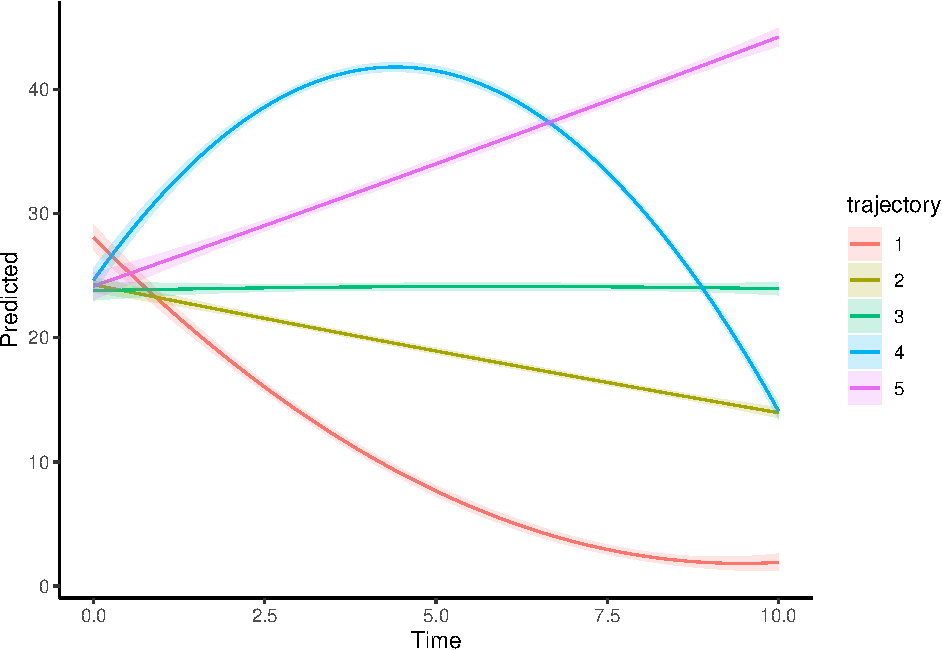
\includegraphics{DZP_R_bookdown_files/figure-latex/unnamed-chunk-36-1.pdf}

Let us check the graph next to the empirical data:

\begin{Shaded}
\begin{Highlighting}[]
\NormalTok{cowplot}\SpecialCharTok{::}\FunctionTok{plot\_grid}\NormalTok{(}\FunctionTok{ggplot}\NormalTok{(}\AttributeTok{data =}\NormalTok{ df, }\FunctionTok{aes}\NormalTok{(}\AttributeTok{x =}\NormalTok{ t, }\AttributeTok{y =}\NormalTok{ y, }\AttributeTok{colour =}\NormalTok{ trajectory)) }\SpecialCharTok{+}
                     \FunctionTok{geom\_point}\NormalTok{() }\SpecialCharTok{+}
                     \FunctionTok{scale\_x\_continuous}\NormalTok{(}\AttributeTok{breaks =}\NormalTok{ t) }\SpecialCharTok{+}
                     \FunctionTok{coord\_cartesian}\NormalTok{(}\AttributeTok{ylim =} \FunctionTok{c}\NormalTok{(}\DecValTok{0}\NormalTok{,}\DecValTok{50}\NormalTok{)) }\SpecialCharTok{+}
                     \FunctionTok{facet\_grid}\NormalTok{(}\AttributeTok{cols =} \FunctionTok{vars}\NormalTok{(trajectory), }\AttributeTok{rows =} \FunctionTok{vars}\NormalTok{(group)) }\SpecialCharTok{+}
                     \FunctionTok{labs}\NormalTok{(}\AttributeTok{colour =} \StringTok{"Trajectory"}\NormalTok{, }\AttributeTok{x =} \StringTok{"Time"}\NormalTok{) }\SpecialCharTok{+}
                     \FunctionTok{theme\_classic}\NormalTok{(),}
                   \FunctionTok{plot\_traj}\NormalTok{(mi, df, }\StringTok{"t"}\NormalTok{), }\AttributeTok{nrow =} \DecValTok{2}\NormalTok{)}
\end{Highlighting}
\end{Shaded}

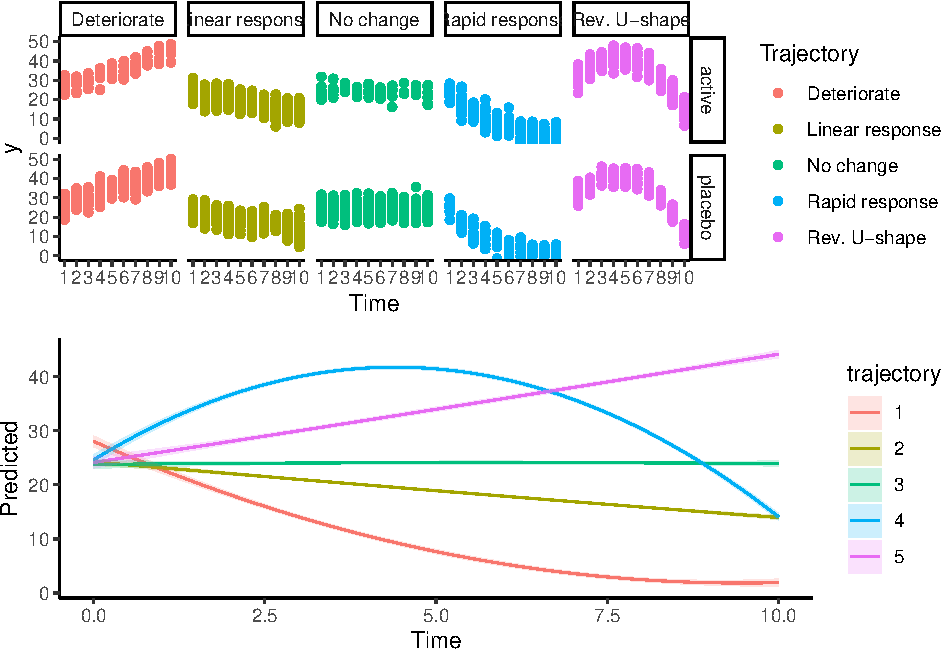
\includegraphics{DZP_R_bookdown_files/figure-latex/unnamed-chunk-37-1.pdf}

\hypertarget{transfer-class-membership-to-original-dataset}{%
\subsection{Transfer class membership to original dataset}\label{transfer-class-membership-to-original-dataset}}

Now we should transfer the determined class to our empirical dataset. Otherwise, we will not be able to run models using the trajectories.

In addition, we extract the certainty, that each person was classified to a category with (the \texttt{pprob} variable in the \texttt{mi} object). Using these probability values we can weigh later models for categorization uncertainty.

Create custom function for transfer:

\begin{Shaded}
\begin{Highlighting}[]
\NormalTok{transfer\_class }\OtherTok{=} \ControlFlowTok{function}\NormalTok{(data, mi)\{}
\NormalTok{  data}\SpecialCharTok{$}\NormalTok{class }\OtherTok{=} \ConstantTok{NA}
  \ControlFlowTok{for}\NormalTok{(ch }\ControlFlowTok{in} \FunctionTok{unique}\NormalTok{(data}\SpecialCharTok{$}\NormalTok{id))\{}
\NormalTok{    data}\SpecialCharTok{$}\NormalTok{class[data}\SpecialCharTok{$}\NormalTok{id }\SpecialCharTok{==}\NormalTok{ ch] }\OtherTok{=}\NormalTok{ mi}\SpecialCharTok{$}\NormalTok{pprob}\SpecialCharTok{$}\NormalTok{class[mi}\SpecialCharTok{$}\NormalTok{pprob}\SpecialCharTok{$}\NormalTok{id }\SpecialCharTok{==}\NormalTok{ ch]}
\NormalTok{    data}\SpecialCharTok{$}\NormalTok{weight[data}\SpecialCharTok{$}\NormalTok{id }\SpecialCharTok{==}\NormalTok{ ch] }\OtherTok{=}\NormalTok{ mi}\SpecialCharTok{$}\NormalTok{pprob[mi}\SpecialCharTok{$}\NormalTok{pprob}\SpecialCharTok{$}\NormalTok{id }\SpecialCharTok{==}\NormalTok{ ch, }\FunctionTok{which}\NormalTok{(}\FunctionTok{grepl}\NormalTok{(}\FunctionTok{paste0}\NormalTok{(}\StringTok{"prob"}\NormalTok{, }\FunctionTok{as.character}\NormalTok{(mi}\SpecialCharTok{$}\NormalTok{pprob}\SpecialCharTok{$}\NormalTok{class[mi}\SpecialCharTok{$}\NormalTok{pprob}\SpecialCharTok{$}\NormalTok{id }\SpecialCharTok{==}\NormalTok{ ch])), }\FunctionTok{colnames}\NormalTok{(mi}\SpecialCharTok{$}\NormalTok{pprob)))]}
\NormalTok{  \}}
\NormalTok{  data}\SpecialCharTok{$}\NormalTok{class }\OtherTok{=} \FunctionTok{factor}\NormalTok{(data}\SpecialCharTok{$}\NormalTok{class)}
  \FunctionTok{return}\NormalTok{(data)}
\NormalTok{\}}
\end{Highlighting}
\end{Shaded}

Transfer data to our original dataframe \texttt{df}:

\begin{Shaded}
\begin{Highlighting}[]
\NormalTok{df }\OtherTok{=} \FunctionTok{transfer\_class}\NormalTok{(}\AttributeTok{data =}\NormalTok{ df, }\AttributeTok{mi =}\NormalTok{ mi)}
\end{Highlighting}
\end{Shaded}

Create data in wide format:

\begin{Shaded}
\begin{Highlighting}[]
\NormalTok{df\_wide }\OtherTok{=} \FunctionTok{as.data.frame}\NormalTok{(df }\SpecialCharTok{\%\textgreater{}\%}
  \FunctionTok{pivot\_wider}\NormalTok{(}\AttributeTok{names\_from =}\NormalTok{ t, }\AttributeTok{values\_from =}\NormalTok{ y))}

\FunctionTok{levels}\NormalTok{(df\_wide}\SpecialCharTok{$}\NormalTok{class) }\OtherTok{=} \FunctionTok{c}\NormalTok{( }\StringTok{"Rapid response"}\NormalTok{,}
                      \StringTok{"Linear response"}\NormalTok{,}
                      \StringTok{"No change"}\NormalTok{,}
                      \StringTok{"Rev. U{-}shape"}\NormalTok{,}
                      \StringTok{"Deteriorate"}\NormalTok{)}
\end{Highlighting}
\end{Shaded}

\hypertarget{modeling-class-membership-as-dependent-variable}{%
\subsection{Modeling class membership as dependent variable}\label{modeling-class-membership-as-dependent-variable}}

We can check the dispersion of the trajectory class variable within the 2 treatment groups using \texttt{table()}:

\begin{Shaded}
\begin{Highlighting}[]
\FunctionTok{table}\NormalTok{(df\_wide}\SpecialCharTok{$}\NormalTok{class, df\_wide}\SpecialCharTok{$}\NormalTok{group)}
\end{Highlighting}
\end{Shaded}

\begin{verbatim}
##                  
##                   active placebo
##   Rapid response      33      12
##   Linear response     90      38
##   No change            8      75
##   Rev. U-shape        35      17
##   Deteriorate          9      33
\end{verbatim}

If we want to use trajectory class membership as the dependent variable, we need to used a logistic-regression model (because \texttt{class} is a categorical variable). Since we usually have more than 2 trajectory classes, we will use a multinomial logistic-regression model.

\begin{Shaded}
\begin{Highlighting}[]
\NormalTok{multinom }\OtherTok{=}\NormalTok{ nnet}\SpecialCharTok{::}\FunctionTok{multinom}\NormalTok{(class }\SpecialCharTok{\textasciitilde{}}\NormalTok{ group, }\AttributeTok{data =}\NormalTok{ df\_wide, }\AttributeTok{weights =}\NormalTok{ weight)}
\end{Highlighting}
\end{Shaded}

\begin{verbatim}
## # weights:  15 (8 variable)
## initial  value 563.055666 
## iter  10 value 471.814704
## final  value 470.947184 
## converged
\end{verbatim}

For an omnibus test, we can use a chi-square-likelihood-ratio test:

\begin{Shaded}
\begin{Highlighting}[]
\NormalTok{car}\SpecialCharTok{::}\FunctionTok{Anova}\NormalTok{(multinom)}
\end{Highlighting}
\end{Shaded}

\begin{verbatim}
## # weights:  10 (4 variable)
## initial  value 563.055666 
## final  value 528.549964 
## converged
\end{verbatim}

\begin{verbatim}
## Analysis of Deviance Table (Type II tests)
## 
## Response: class
##       LR Chisq Df Pr(>Chisq)    
## group   115.21  4  < 2.2e-16 ***
## ---
## Signif. codes:  0 '***' 0.001 '**' 0.01 '*' 0.05 '.' 0.1 ' ' 1
\end{verbatim}

For pairwise comparisons we can use the \texttt{emmeans} package:

\begin{Shaded}
\begin{Highlighting}[]
\NormalTok{emmeans}\SpecialCharTok{::}\FunctionTok{lsmeans}\NormalTok{(multinom, pairwise }\SpecialCharTok{\textasciitilde{}}\NormalTok{ group }\SpecialCharTok{|}\NormalTok{ class, }\AttributeTok{adjust=}\StringTok{"tukey"}\NormalTok{, }\AttributeTok{mode =} \StringTok{"prob"}\NormalTok{)}
\end{Highlighting}
\end{Shaded}

\begin{verbatim}
## $lsmeans
## class = Rapid response:
##  group     prob     SE df lower.CL upper.CL
##  active  0.1887 0.0296  8  0.12049   0.2570
##  placebo 0.0686 0.0191  8  0.02452   0.1126
## 
## class = Linear response:
##  group     prob     SE df lower.CL upper.CL
##  active  0.5139 0.0378  8  0.42671   0.6010
##  placebo 0.2171 0.0312  8  0.14527   0.2890
## 
## class = No change:
##  group     prob     SE df lower.CL upper.CL
##  active  0.0458 0.0158  8  0.00931   0.0822
##  placebo 0.4286 0.0374  8  0.34230   0.5148
## 
## class = Rev. U-shape:
##  group     prob     SE df lower.CL upper.CL
##  active  0.2002 0.0303  8  0.13039   0.2699
##  placebo 0.0971 0.0224  8  0.04552   0.1488
## 
## class = Deteriorate:
##  group     prob     SE df lower.CL upper.CL
##  active  0.0515 0.0167  8  0.01294   0.0900
##  placebo 0.1886 0.0296  8  0.12039   0.2568
## 
## Confidence level used: 0.95 
## 
## $contrasts
## class = Rapid response:
##  contrast         estimate     SE df t.ratio p.value
##  active - placebo    0.120 0.0352  8   3.411  0.0092
## 
## class = Linear response:
##  contrast         estimate     SE df t.ratio p.value
##  active - placebo    0.297 0.0490  8   6.057  0.0003
## 
## class = No change:
##  contrast         estimate     SE df t.ratio p.value
##  active - placebo   -0.383 0.0406  8  -9.427  <.0001
## 
## class = Rev. U-shape:
##  contrast         estimate     SE df t.ratio p.value
##  active - placebo    0.103 0.0376  8   2.737  0.0256
## 
## class = Deteriorate:
##  contrast         estimate     SE df t.ratio p.value
##  active - placebo   -0.137 0.0340  8  -4.037  0.0038
\end{verbatim}

Estimates are displayed as log-odds, so we have to exponentiate them using \texttt{exp()} to get interpretable odds ratios (OR).

\hypertarget{determine-the-optimal-model}{%
\subsection{Determine the optimal model}\label{determine-the-optimal-model}}

In the previous dataset, we have

\begin{enumerate}
\def\labelenumi{\arabic{enumi}.}
\tightlist
\item
  used a qudratic polynomial
\item
  extracted 5 groups
\item
  allowed free variation of the intercept as the random effect.
\end{enumerate}

However, usually we operate on a more data-driven approach, i.e.~without knowing these parameters in advance.

There are several statistical criteria to determine a mode that optimally describes the data. For LCLMM, the most commonly used ones are:

\begin{itemize}
\tightlist
\item
  Bayesian Information Criterion (BIC)

  \begin{itemize}
  \tightlist
  \item
    lower values on these information criteria indicate better fitting models
  \item
    models that do not fit better than the baseline model can be dismissed, and a selection of the best fitting models can be carried forward and examined further
  \end{itemize}
\item
  Entropy

  \begin{itemize}
  \tightlist
  \item
    ranges from 0.00 to 1.00
  \item
    high values of entropy (\textgreater{} .80) indicate that individuals are classified with confidence
  \item
    models with higher entropy are favored
  \end{itemize}
\item
  Adjusted Lo-Mendell-Rubin likelihood ratio test

  \begin{itemize}
  \tightlist
  \item
    corrected likelihood-ratio distribution (a chi-square distribution is inappropriate) to compare models with C and C -- 1 unobserved groups
  \item
    likelihood ratio tests compare models that differ only in the number of classes
  \item
    significance test (p\textless{} .05) indicates that the model with C -- 1 classes should be rejected in favor of the model with C classes
  \end{itemize}
\end{itemize}

\hypertarget{selection-loop}{%
\subsection{Selection loop}\label{selection-loop}}

To try this, let us run a model selection based on the Bayesian Information Criterion (BIC).

Since we have to test a lot of parameters, we run the model fitting procedure in a loop and save the results in a container:

This procedure can take quite a while, so we'll test it in a smaller dataset:

\begin{Shaded}
\begin{Highlighting}[]
\NormalTok{test }\OtherTok{=} \FunctionTok{read.csv}\NormalTok{(}\StringTok{"https://raw.githubusercontent.com/stephangoerigk/DZP\_Workshop\_Slides/master/test.csv"}\NormalTok{)}
\end{Highlighting}
\end{Shaded}

Inspect the data:

\begin{Shaded}
\begin{Highlighting}[]
\NormalTok{psych}\SpecialCharTok{::}\FunctionTok{describe}\NormalTok{(test)}
\end{Highlighting}
\end{Shaded}

\begin{verbatim}
##        vars    n   mean     sd median trimmed    mad   min    max  range  skew
## X         1 1680 200.29 113.20  219.4  204.98 150.48  1.00 352.80 351.80 -0.26
## group*    2 1680   1.50   0.50    1.5    1.50   0.74  1.00   2.00   1.00  0.00
## t         3 1680   4.50   2.87    4.5    4.50   3.71  0.00   9.00   9.00  0.00
## stress    4 1677  43.39  30.65   48.0   42.29  39.56 -2.79 101.98 104.77  0.14
## id        5 1680 200.02 113.20  219.0  204.71 150.48  1.00 352.00 351.00 -0.26
##        kurtosis   se
## X         -1.38 2.76
## group*    -2.00 0.01
## t         -1.23 0.07
## stress    -1.07 0.75
## id        -1.38 2.76
\end{verbatim}

\begin{Shaded}
\begin{Highlighting}[]
\FunctionTok{head}\NormalTok{(test)}
\end{Highlighting}
\end{Shaded}

\begin{verbatim}
##      X   group t    stress id
## 1 39.0 Healthy 0 80.199113 39
## 2 39.2 Healthy 1 70.188702 39
## 3 39.4 Healthy 2 50.653667 39
## 4 39.6 Healthy 3 16.588692 39
## 5 39.8 Healthy 4 -2.031454 39
## 6 39.1 Healthy 5 -1.285336 39
\end{verbatim}

Let us first set up a container:

\begin{Shaded}
\begin{Highlighting}[]
\NormalTok{results\_total }\OtherTok{=} \FunctionTok{data.frame}\NormalTok{(}\AttributeTok{ng =} \ConstantTok{NA}\NormalTok{,}
                           \AttributeTok{Polynomial =} \ConstantTok{NA}\NormalTok{,}
                           \AttributeTok{Random =} \ConstantTok{NA}\NormalTok{,}
                           \AttributeTok{BIC =} \ConstantTok{NA}\NormalTok{,}
                           \AttributeTok{AIC =} \ConstantTok{NA}\NormalTok{,}
                           \AttributeTok{loglik =} \ConstantTok{NA}\NormalTok{)}
\end{Highlighting}
\end{Shaded}

We will run out loop for 2:5 groups,quadratic vs.~cubic polynomial and different random effect compositions:

\begin{Shaded}
\begin{Highlighting}[]
\FunctionTok{set.seed}\NormalTok{(}\DecValTok{222}\NormalTok{)}

\ControlFlowTok{for}\NormalTok{(ng }\ControlFlowTok{in} \DecValTok{2}\SpecialCharTok{:}\DecValTok{5}\NormalTok{)\{}
  \ControlFlowTok{for}\NormalTok{(random }\ControlFlowTok{in} \FunctionTok{c}\NormalTok{(}\StringTok{"\textasciitilde{} 1"}\NormalTok{, }\StringTok{"\textasciitilde{} 1 + t"}\NormalTok{))\{}
\NormalTok{    mi\_sq }\OtherTok{\textless{}{-}}\NormalTok{ lcmm}\SpecialCharTok{::}\FunctionTok{hlme}\NormalTok{(}\AttributeTok{fixed =}\NormalTok{ stress }\SpecialCharTok{\textasciitilde{}} \DecValTok{1} \SpecialCharTok{+}\NormalTok{ t }\SpecialCharTok{+} \FunctionTok{I}\NormalTok{(t}\SpecialCharTok{\^{}}\DecValTok{2}\NormalTok{),}
                        \AttributeTok{mixture =} \SpecialCharTok{\textasciitilde{}} \DecValTok{1} \SpecialCharTok{+}\NormalTok{ t }\SpecialCharTok{+} \FunctionTok{I}\NormalTok{(t}\SpecialCharTok{\^{}}\DecValTok{2}\NormalTok{),}
                        \AttributeTok{random =} \FunctionTok{as.formula}\NormalTok{(random),}
                        \AttributeTok{ng =}\NormalTok{ ng,}
                        \AttributeTok{nwg =} \ConstantTok{FALSE}\NormalTok{,}
                        \AttributeTok{idiag =} \ConstantTok{FALSE}\NormalTok{,}
                        \AttributeTok{data =}\NormalTok{ test,}
                        \AttributeTok{subject =} \StringTok{"id"}\NormalTok{)}
\NormalTok{    mi\_cub }\OtherTok{\textless{}{-}}\NormalTok{ lcmm}\SpecialCharTok{::}\FunctionTok{hlme}\NormalTok{(}\AttributeTok{fixed =}\NormalTok{ stress }\SpecialCharTok{\textasciitilde{}} \DecValTok{1} \SpecialCharTok{+}\NormalTok{ t }\SpecialCharTok{+} \FunctionTok{I}\NormalTok{(t}\SpecialCharTok{\^{}}\DecValTok{3}\NormalTok{),}
                         \AttributeTok{mixture =} \SpecialCharTok{\textasciitilde{}} \DecValTok{1} \SpecialCharTok{+}\NormalTok{ t }\SpecialCharTok{+} \FunctionTok{I}\NormalTok{(t}\SpecialCharTok{\^{}}\DecValTok{3}\NormalTok{),}
                         \AttributeTok{random =} \FunctionTok{as.formula}\NormalTok{(random),}
                         \AttributeTok{ng =}\NormalTok{ ng,}
                         \AttributeTok{nwg =} \ConstantTok{FALSE}\NormalTok{,}
                         \AttributeTok{idiag =} \ConstantTok{FALSE}\NormalTok{,}
                         \AttributeTok{data =}\NormalTok{ test,}
                         \AttributeTok{subject =} \StringTok{"id"}\NormalTok{)}

\NormalTok{    sq }\OtherTok{\textless{}{-}} \FunctionTok{c}\NormalTok{(mi\_sq}\SpecialCharTok{$}\NormalTok{ng, }\DecValTok{2}\NormalTok{, random, mi\_sq}\SpecialCharTok{$}\NormalTok{BIC, mi\_sq}\SpecialCharTok{$}\NormalTok{AIC, mi\_sq}\SpecialCharTok{$}\NormalTok{loglik)}
\NormalTok{    cub }\OtherTok{\textless{}{-}} \FunctionTok{c}\NormalTok{(mi\_cub}\SpecialCharTok{$}\NormalTok{ng, }\DecValTok{3}\NormalTok{, random, mi\_cub}\SpecialCharTok{$}\NormalTok{BIC, mi\_cub}\SpecialCharTok{$}\NormalTok{AIC, mi\_cub}\SpecialCharTok{$}\NormalTok{loglik)}
\NormalTok{    results\_total }\OtherTok{=} \FunctionTok{rbind}\NormalTok{(results\_total, sq)}
\NormalTok{    results\_total }\OtherTok{=} \FunctionTok{rbind}\NormalTok{(results\_total, cub)}
\NormalTok{  \}}
\NormalTok{\}}

\NormalTok{results\_total }\OtherTok{=}\NormalTok{ results\_total[}\FunctionTok{order}\NormalTok{(results\_total}\SpecialCharTok{$}\NormalTok{BIC, }\AttributeTok{decreasing =}\NormalTok{ T),]}
\end{Highlighting}
\end{Shaded}

The solution with the lowest BIC is chosen. Now we can once more fit the LCLMM, only now we used the determined parameters

CAVE: While a statistical determination of model parameters is important, there should always be clinical plausibility checks as well.

  \bibliography{book.bib,packages.bib}

\end{document}
